\section{投影相机模型}\label{sec:投影相机模型}

三维计算机图形学中的一个基本问题是{\itshape 3D视见问题}:
如何将三维场景投影到二维图像上进行显示。
大多数经典方法都可以用$4\times4$的\keyindex{投影变换}{projective transformation}{transformation变换}矩阵来表达。
因此,我们将引入一个投影矩阵相机类\refvar{ProjectiveCamera}{},
然后在此基础上定义两个相机模型。
第一个实现了\keyindex{正交投影}{orthographic projection}{projection投影},
另一个实现了\keyindex{透视投影}{perspective projection}{projection投影}——
两种经典且广泛使用的\keyindex{投影}{projection}{}。
\begin{lstlisting}
`\initcode{Camera Declarations}{+=}\lastcode{CameraDeclarations}`
class `\initvar{ProjectiveCamera}{}` : public `\refvar{Camera}{}` {
public:
    `\refcode{ProjectiveCamera Public Methods}{}`
protected:
    `\refcode{ProjectiveCamera Protected Data}{}`
};
\end{lstlisting}

还有三个坐标系(总结于\reffig{6.1}中)对定义和讨论投影相机很有用。
\begin{itemize}
    \item \keyindex{屏幕空间}{screen space}{}:
          屏幕空间定义在胶片平面上。相机将相机空间中的物体投影到胶片平面上;
          \keyindex{屏幕窗口}{screen window}{}内的部分在生成的图像中是可见的。
          屏幕空间的深度$z$值从0变到1,分别对应近处和远处截平面的点。
          注意,虽然这称为“屏幕”空间,但它仍然是一个三维坐标系,因为$z$值是有意义的。
    \item \keyindex{规范化设备坐标}{normalized device coordinate}{}(NDC){\sffamily 空间}:
          这是被渲染的实际图像的坐标系。对于$x$和$y$,该空间范围从$(0,0)$变到$(1,1)$,
          其中$(0,0)$是图像的左上角。深度值与屏幕空间中的相同,线性变换将屏幕空间转换为NDC空间。
    \item \keyindex{栅格空间}{raster space}{}\sidenote{译者注:也称光栅空间。}:
          这与NDC空间几乎相同,除了$x$和$y$坐标从$(0,0)$变到(resolution.x, resolution.y)
          \sidenote{译者注:resolution指分辨率。}。
\end{itemize}

投影相机用$4\times4$矩阵在所有这些空间之间进行转换,
但具有特殊成像特性的相机不必用矩阵表示所有这些转换。
\begin{figure}[htbp]
    \centering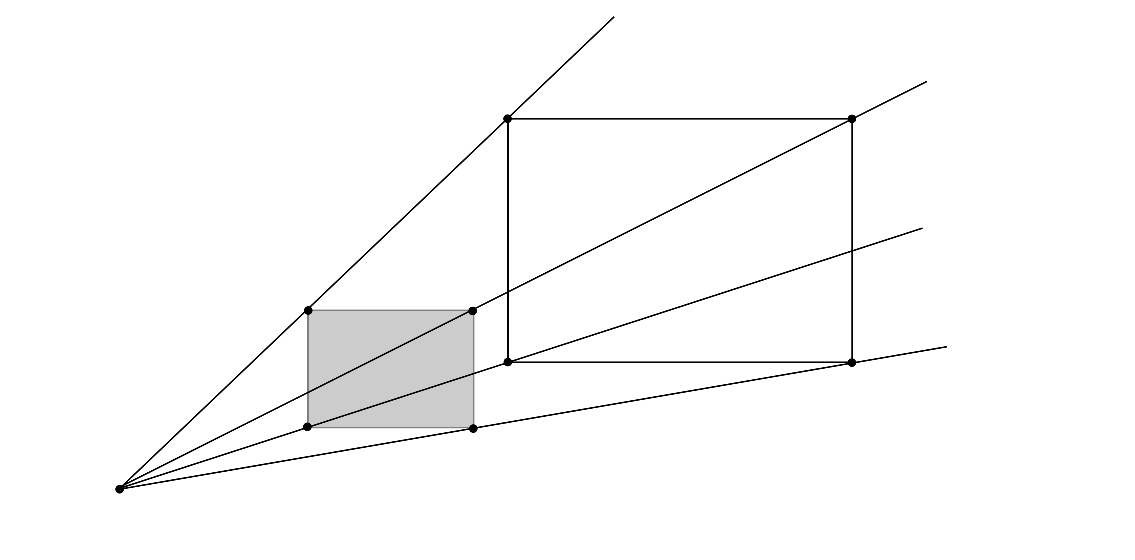
\includegraphics[width=0.75\linewidth]{chap06/Cameracoordinatespaces.eps}
    \put(-280,0){\small 相机空间:$(0,0,0)$}
    \put(-270,60){\small NDC:$(0,0,0)$}
    \put(-220,110){\small NDC:$(0,0,1)$}
    \put(-160,20){\small $z=\text{near}$}
    \put(-160,10){\small NDC:$(1,1,0)$}
    \put(-160,0){\small 栅格:$(\text{res}.x,\text{res}.y,0)$}
    \put(-70,35){\small $z=\text{far}$}
    \put(-70,25){\small NDC:$(1,1,1)$}
    \put(-70,15){\small 栅格:$(\text{res}.x,\text{res}.y,1)$}
    \caption{几个与相机相关的坐标空间常用于简化\protect\refvar{Camera}{}的实现。
        相机类持有它们之间的变换。世界空间中的场景物体由相机查看,它位于相机空间原点,并指向$+z$轴。
        近处和远处平面之间的物体被投影到相机空间中的胶片平面$z=\text{near}$上。
        胶片平面在栅格空间中$z=0$处,其中$x$和$y$范围从$(0,0)$变到(resolution.x, resolution.y)。
        规范化设备坐标(NDC)空间将栅格空间归一化,因此$x$和$y$范围从$(0,0)$变到$(1,1)$。}
    \label{fig:6.1}
\end{figure}

除了基类\refvar{Camera}{}要求的参数外,\refvar{ProjectiveCamera}{}还接收投影变换矩阵、
图像的屏幕空间范围以及与景深有关的额外参数。
\keyindex{景深}{depth of field}{}将在本节末尾介绍和实现,
它模拟了真实透镜系统中出现的失焦物体的模糊性。
\begin{lstlisting}
`\initcode{ProjectiveCamera Public Methods}{=}`
`\refvar{ProjectiveCamera}{}`(const `\refvar{AnimatedTransform}{}` &CameraToWorld, 
        const `\refvar{Transform}{}` &CameraToScreen, const `\refvar{Bounds2f}{}` &screenWindow,
        `\refvar{Float}{}` shutterOpen, `\refvar{Float}{}` shutterClose, `\refvar{Float}{}` lensr, `\refvar{Float}{}` focald,
        `\refvar{Film}{}` *film, const `\refvar{Medium}{}` *medium)
    : `\refvar{Camera}{}`(CameraToWorld, shutterOpen, shutterClose, film, medium),
      `\refvar{CameraToScreen}{}`(CameraToScreen) {
    `\refcode{Initialize depth of field parameters}{}`
    `\refcode{Compute projective camera transformations}{}`
}
\end{lstlisting}

\refvar{ProjectiveCamera}{}的实现将投影变换传递给这里展示的基类构造函数。
该变换给出了相机到屏幕的投影;
由此,构造函数能轻松算出从栅格空间到相机空间一路所需的其他变换。
\begin{lstlisting}
`\initcode{Compute projective camera transformations}{=}`
`\refcode{Compute projective camera screen transformations}{}`
`\refvar{RasterToCamera}{}` = `\refvar[Transform::Inverse]{Inverse}{}`(CameraToScreen) * `\refvar{RasterToScreen}{}`;
\end{lstlisting}
\begin{lstlisting}
`\initcode{ProjectiveCamera Protected Data}{=}\initnext{ProjectiveCameraProtectedData}`
`\refvar{Transform}{}` `\initvar{CameraToScreen}{}`, `\initvar{RasterToCamera}{}`;
\end{lstlisting}

在构造函数中唯一要计算的重要变换是屏幕到栅格的投影。
在下面的代码中,请注意变换的组成(从下往上看),
我们从屏幕空间的一个点开始,先平移使得屏幕左上角位于原点,
然后用屏幕宽度和高度的倒数进行缩放,
得到一个$x$和$y$坐标在0到1之间的点(这些是NDC坐标)。
最后,我们用栅格化分辨率进行缩放,这样我们最终就能完全覆盖
从$(0,0)$直到整个栅格分辨率的栅格范围。
这里一个重要细节是$y$坐标被该变换倒置了;
这是必要的,因为增加的$y$值在屏幕坐标中是向上移动但在栅格坐标中是向下的。
\begin{lstlisting}
`\initcode{Compute projective camera screen transformations}{=}`
`\refvar{ScreenToRaster}{}` = `\refvar{Scale}{}`(film->`\refvar{fullResolution}{}`.x, 
                       film->`\refvar{fullResolution}{}`.y, 1) *
    `\refvar{Scale}{}`(1 / (screenWindow.`\refvar{pMax}{}`.x - screenWindow.`\refvar{pMin}{}`.x),
          1 / (screenWindow.`\refvar{pMin}{}`.y - screenWindow.`\refvar{pMax}{}`.y), 1) *
    `\refvar{Translate}{}`(`\refvar{Vector3f}{}`(-screenWindow.`\refvar{pMin}{}`.x, -screenWindow.`\refvar{pMax}{}`.y, 0));
`\refvar{RasterToScreen}{}` = `\refvar[Transform::Inverse]{Inverse}{}`(`\refvar{ScreenToRaster}{}`);
\end{lstlisting}
\begin{lstlisting}
`\refcode{ProjectiveCamera Protected Data}{+=}\lastnext{ProjectiveCameraProtectedData}`
`\refvar{Transform}{}` `\initvar{ScreenToRaster}{}`, `\initvar{RasterToScreen}{}`;
\end{lstlisting}

\subsection{正交相机}\label{sub:正交相机}
\begin{lstlisting}
`\initcode{OrthographicCamera Declarations}{=}`
class `\initvar{OrthographicCamera}{}` : public `\refvar{ProjectiveCamera}{}` {
public:
    `\refcode{OrthographicCamera Public Methods}{}`
private:
    `\refcode{OrthographicCamera Private Data}{}`
};
\end{lstlisting}

定义在文件\href{https://github.com/mmp/pbrt-v3/blob/master/src/cameras/orthographic.h}{\ttfamily cameras/orthographic.h}和
\href{https://github.com/mmp/pbrt-v3/tree/master/src/cameras/orthographic.cpp}{\ttfamily cameras/orthographic.cpp}中的\keyindex{正交相机}{orthographic camera}{camera相机},
是基于正交投影变换的。
正交变换取场景中的一块矩形区域并将其投影到定义该区域之框的前方一面。
它不具有\keyindex{前缩}{foreshortening}{}效应——当物体远离时它们在成像平面上变小——
但它让平行线依然平行,并保留物体间的相对距离。
\reffig{6.2}{}展示了该立方体是如何定义场景可见区域的。
\begin{figure}[htbp]
    \centering%LaTeX with PSTricks extensions
%%Creator: Inkscape 1.1.1 (3bf5ae0d25, 2021-09-20)
%%Please note this file requires PSTricks extensions
\psset{xunit=.5pt,yunit=.5pt,runit=.5pt}
\begin{pspicture}(254.52000427,244.36999512)
{
\newrgbcolor{curcolor}{0 0 0}
\pscustom[linewidth=1,linecolor=curcolor]
{
\newpath
\moveto(5.5,162.19999512)
\lineto(5.5,8.15999512)
\lineto(160.1,8.15999512)
}
}
{
\newrgbcolor{curcolor}{0 0 0}
\pscustom[linestyle=none,fillstyle=solid,fillcolor=curcolor]
{
\newpath
\moveto(0,157.28999512)
\lineto(5.5,161.54999512)
\lineto(11.01,157.28999512)
\lineto(5.5,170.29999512)
\closepath
}
}
{
\newrgbcolor{curcolor}{0.65098041 0.65098041 0.65098041}
\pscustom[linestyle=none,fillstyle=solid,fillcolor=curcolor]
{
\newpath
\moveto(1.2,158.84999512)
\lineto(5.5,168.98999512)
\lineto(5.5,162.17999512)
\closepath
}
}
{
\newrgbcolor{curcolor}{0.40000001 0.40000001 0.40000001}
\pscustom[linestyle=none,fillstyle=solid,fillcolor=curcolor]
{
\newpath
\moveto(9.8,158.84999512)
\lineto(5.5,168.98999512)
\lineto(5.5,162.17999512)
\closepath
}
}
{
\newrgbcolor{curcolor}{0 0 0}
\pscustom[linestyle=none,fillstyle=solid,fillcolor=curcolor]
{
\newpath
\moveto(155.19,2.65999512)
\lineto(159.45,8.15999512)
\lineto(155.19,13.66999512)
\lineto(168.21,8.15999512)
\closepath
}
}
{
\newrgbcolor{curcolor}{0.65098041 0.65098041 0.65098041}
\pscustom[linestyle=none,fillstyle=solid,fillcolor=curcolor]
{
\newpath
\moveto(156.75,3.85999512)
\lineto(166.89,8.15999512)
\lineto(160.08,8.15999512)
\closepath
}
}
{
\newrgbcolor{curcolor}{0.40000001 0.40000001 0.40000001}
\pscustom[linestyle=none,fillstyle=solid,fillcolor=curcolor]
{
\newpath
\moveto(156.75,12.45999512)
\lineto(166.89,8.15999512)
\lineto(160.08,8.15999512)
\closepath
}
}
{
\newrgbcolor{curcolor}{0 0 0}
\pscustom[linewidth=1,linecolor=curcolor]
{
\newpath
\moveto(218.6000061,221.28999519)
\lineto(5.51999998,8.20999146)
}
}
{
\newrgbcolor{curcolor}{0 0 0}
\pscustom[linestyle=none,fillstyle=solid,fillcolor=curcolor]
{
\newpath
\moveto(211.24,221.70999512)
\lineto(218.14,220.82999512)
\lineto(219.02,213.92999512)
\lineto(224.33,227.01999512)
\closepath
}
}
{
\newrgbcolor{curcolor}{0.65098041 0.65098041 0.65098041}
\pscustom[linestyle=none,fillstyle=solid,fillcolor=curcolor]
{
\newpath
\moveto(213.19,221.95999512)
\lineto(223.4,226.08999512)
\lineto(218.59,221.27999512)
\closepath
}
}
{
\newrgbcolor{curcolor}{0.40000001 0.40000001 0.40000001}
\pscustom[linestyle=none,fillstyle=solid,fillcolor=curcolor]
{
\newpath
\moveto(219.27,215.87999512)
\lineto(223.4,226.08999512)
\lineto(218.59,221.27999512)
\closepath
}
}
{
\newrgbcolor{curcolor}{0.60000002 0.60000002 0.60000002}
\pscustom[linestyle=none,fillstyle=solid,fillcolor=curcolor]
{
\newpath
\moveto(62.79000092,116.37999725)
\lineto(172.98000336,116.37999725)
\lineto(172.98000336,50.18000031)
\lineto(62.79000092,50.18000031)
\closepath
}
}
{
\newrgbcolor{curcolor}{0 0 0}
\pscustom[linewidth=1,linecolor=curcolor]
{
\newpath
\moveto(62.79000092,116.37999725)
\lineto(172.98000336,116.37999725)
\lineto(172.98000336,50.18000031)
\lineto(62.79000092,50.18000031)
\closepath
}
}
{
\newrgbcolor{curcolor}{0 0 0}
\pscustom[linewidth=1,linecolor=curcolor,linestyle=dashed,dash=2]
{
\newpath
\moveto(254.02,131.03999512)
\lineto(143.83,131.03999512)
\lineto(143.83,197.23999512)
}
}
{
\newrgbcolor{curcolor}{0 0 0}
\pscustom[linewidth=1,linecolor=curcolor]
{
\newpath
\moveto(143.83,197.23999512)
\lineto(254.02,197.23999512)
\lineto(254.02,131.03999512)
}
}
{
\newrgbcolor{curcolor}{0 0 0}
\pscustom[linewidth=1,linecolor=curcolor]
{
\newpath
\moveto(62.79000092,116.37999725)
\lineto(143.83000183,197.23999405)
}
}
{
\newrgbcolor{curcolor}{0.60000002 0.60000002 0.60000002}
\pscustom[linestyle=none,fillstyle=solid,fillcolor=curcolor]
{
\newpath
\moveto(172.97999573,116.37999725)
\lineto(254.02000427,197.23999405)
}
}
{
\newrgbcolor{curcolor}{0 0 0}
\pscustom[linewidth=1,linecolor=curcolor]
{
\newpath
\moveto(172.97999573,116.37999725)
\lineto(254.02000427,197.23999405)
}
}
{
\newrgbcolor{curcolor}{0.60000002 0.60000002 0.60000002}
\pscustom[linestyle=none,fillstyle=solid,fillcolor=curcolor]
{
\newpath
\moveto(254.02000427,131.03999329)
\lineto(172.97999573,50.17999268)
}
}
{
\newrgbcolor{curcolor}{0 0 0}
\pscustom[linewidth=1,linecolor=curcolor]
{
\newpath
\moveto(254.02000427,131.03999329)
\lineto(172.97999573,50.17999268)
}
}
{
\newrgbcolor{curcolor}{0.60000002 0.60000002 0.60000002}
\pscustom[linestyle=none,fillstyle=solid,fillcolor=curcolor]
{
\newpath
\moveto(143.83000183,131.03999329)
\lineto(62.79000092,50.17999268)
}
}
{
\newrgbcolor{curcolor}{0 0 0}
\pscustom[linewidth=1,linecolor=curcolor,linestyle=dashed,dash=2]
{
\newpath
\moveto(143.83000183,131.03999329)
\lineto(62.79000092,50.17999268)
}
}
{
\newrgbcolor{curcolor}{0 0 0}
\pscustom[linestyle=none,fillstyle=solid,fillcolor=curcolor]
{
\newpath
\moveto(230.6197021,224.91641024)
\curveto(231.6822021,226.07266024)(232.2759521,226.57266024)(232.9947021,227.19766024)
\curveto(232.9947021,227.19766024)(234.2134521,228.26016024)(234.9322021,228.97891024)
\curveto(236.8384521,230.82266024)(237.2759521,231.79141024)(237.2759521,231.88516024)
\curveto(237.2759521,232.07266024)(237.0884521,232.07266024)(237.0572021,232.07266024)
\curveto(236.9009521,232.07266024)(236.8697021,232.04141024)(236.7447021,231.85391024)
\curveto(236.1509521,230.88516024)(235.7447021,230.57266024)(235.2759521,230.57266024)
\curveto(234.7759521,230.57266024)(234.5572021,230.88516024)(234.2447021,231.22891024)
\curveto(233.8697021,231.66641024)(233.5259521,232.07266024)(232.8697021,232.07266024)
\curveto(231.3697021,232.07266024)(230.4634521,230.22891024)(230.4634521,229.79141024)
\curveto(230.4634521,229.69766024)(230.5259521,229.57266024)(230.6822021,229.57266024)
\curveto(230.8697021,229.57266024)(230.9009521,229.66641024)(230.9634521,229.79141024)
\curveto(231.3384521,230.72891024)(232.4947021,230.72891024)(232.6509521,230.72891024)
\curveto(233.0572021,230.72891024)(233.4322021,230.60391024)(233.9009521,230.44766024)
\curveto(234.7134521,230.13516024)(234.9322021,230.13516024)(235.4322021,230.13516024)
\curveto(234.7134521,229.29141024)(233.0572021,227.85391024)(232.6822021,227.54141024)
\lineto(230.8697021,225.85391024)
\curveto(229.5259521,224.51016024)(228.8072021,223.38516024)(228.8072021,223.22891024)
\curveto(228.8072021,223.04141024)(229.0259521,223.04141024)(229.0572021,223.04141024)
\curveto(229.2134521,223.04141024)(229.2447021,223.07266024)(229.3697021,223.29141024)
\curveto(229.8384521,224.01016024)(230.4322021,224.54141024)(231.0884521,224.54141024)
\curveto(231.5259521,224.54141024)(231.7447021,224.35391024)(232.2447021,223.79141024)
\curveto(232.5572021,223.35391024)(232.9322021,223.04141024)(233.4947021,223.04141024)
\curveto(235.4947021,223.04141024)(236.6509521,225.57266024)(236.6509521,226.10391024)
\curveto(236.6509521,226.19766024)(236.5572021,226.32266024)(236.4009521,226.32266024)
\curveto(236.2134521,226.32266024)(236.1822021,226.19766024)(236.1197021,226.04141024)
\curveto(235.6509521,224.76016024)(234.3697021,224.38516024)(233.7134521,224.38516024)
\curveto(233.3384521,224.38516024)(232.9634521,224.51016024)(232.5572021,224.63516024)
\curveto(231.8697021,224.88516024)(231.5572021,224.97891024)(231.1509521,224.97891024)
\curveto(231.1197021,224.97891024)(230.8072021,224.97891024)(230.6197021,224.91641024)
\closepath
\moveto(230.6197021,224.91641024)
}
}
{
\newrgbcolor{curcolor}{0 0 0}
\pscustom[linestyle=none,fillstyle=solid,fillcolor=curcolor]
{
\newpath
\moveto(178.4398241,10.53037624)
\curveto(178.5648241,11.03037624)(179.0335741,12.87412624)(180.4085741,12.87412624)
\curveto(180.5023241,12.87412624)(181.0023241,12.87412624)(181.4085741,12.62412624)
\curveto(180.8460741,12.49912624)(180.4710741,12.03037624)(180.4710741,11.53037624)
\curveto(180.4710741,11.21787624)(180.6898241,10.84287624)(181.2210741,10.84287624)
\curveto(181.6585741,10.84287624)(182.2835741,11.18662624)(182.2835741,11.99912624)
\curveto(182.2835741,13.03037624)(181.1273241,13.31162624)(180.4398241,13.31162624)
\curveto(179.2835741,13.31162624)(178.5960741,12.24912624)(178.3460741,11.81162624)
\curveto(177.8460741,13.12412624)(176.7835741,13.31162624)(176.1898241,13.31162624)
\curveto(174.1273241,13.31162624)(172.9710741,10.74912624)(172.9710741,10.24912624)
\curveto(172.9710741,10.03037624)(173.1898241,10.03037624)(173.2210741,10.03037624)
\curveto(173.3773241,10.03037624)(173.4398241,10.09287624)(173.4710741,10.24912624)
\curveto(174.1585741,12.37412624)(175.4710741,12.87412624)(176.1585741,12.87412624)
\curveto(176.5335741,12.87412624)(177.2210741,12.68662624)(177.2210741,11.53037624)
\curveto(177.2210741,10.90537624)(176.8773241,9.59287624)(176.1585741,6.78037624)
\curveto(175.8460741,5.56162624)(175.1273241,4.71787624)(174.2523241,4.71787624)
\curveto(174.1273241,4.71787624)(173.6898241,4.71787624)(173.2523241,4.96787624)
\curveto(173.7523241,5.09287624)(174.1898241,5.49912624)(174.1898241,6.06162624)
\curveto(174.1898241,6.59287624)(173.7523241,6.74912624)(173.4710741,6.74912624)
\curveto(172.8460741,6.74912624)(172.3773241,6.24912624)(172.3773241,5.59287624)
\curveto(172.3773241,4.68662624)(173.3460741,4.28037624)(174.2210741,4.28037624)
\curveto(175.5648241,4.28037624)(176.2835741,5.68662624)(176.3148241,5.78037624)
\curveto(176.5648241,5.06162624)(177.2835741,4.28037624)(178.4710741,4.28037624)
\curveto(180.5335741,4.28037624)(181.6585741,6.84287624)(181.6585741,7.34287624)
\curveto(181.6585741,7.56162624)(181.5023241,7.56162624)(181.4398241,7.56162624)
\curveto(181.2523241,7.56162624)(181.2210741,7.46787624)(181.1585741,7.34287624)
\curveto(180.5023241,5.18662624)(179.1585741,4.71787624)(178.5335741,4.71787624)
\curveto(177.7523241,4.71787624)(177.4398241,5.34287624)(177.4398241,6.03037624)
\curveto(177.4398241,6.46787624)(177.5335741,6.90537624)(177.7523241,7.78037624)
\closepath
\moveto(178.4398241,10.53037624)
}
}
{
\newrgbcolor{curcolor}{0 0 0}
\pscustom[linestyle=none,fillstyle=solid,fillcolor=curcolor]
{
\newpath
\moveto(12.9314461,185.17229724)
\curveto(13.0251961,185.45354724)(13.0251961,185.48479724)(13.0251961,185.64104724)
\curveto(13.0251961,185.98479724)(12.7439461,186.17229724)(12.4314461,186.17229724)
\curveto(12.2439461,186.17229724)(11.9314461,186.04729724)(11.7439461,185.76604724)
\curveto(11.7126961,185.64104724)(11.5251961,185.04729724)(11.4626961,184.67229724)
\curveto(11.3064461,184.17229724)(11.1814461,183.60979724)(11.0564461,183.07854724)
\lineto(10.1501961,179.48479724)
\curveto(10.0876961,179.20354724)(9.2126961,177.79729724)(7.9001961,177.79729724)
\curveto(6.9001961,177.79729724)(6.6814461,178.67229724)(6.6814461,179.42229724)
\curveto(6.6814461,180.32854724)(7.0251961,181.57854724)(7.6814461,183.32854724)
\curveto(7.9939461,184.14104724)(8.0876961,184.35979724)(8.0876961,184.76604724)
\curveto(8.0876961,185.64104724)(7.4626961,186.39104724)(6.4626961,186.39104724)
\curveto(4.5564461,186.39104724)(3.8376961,183.48479724)(3.8376961,183.32854724)
\curveto(3.8376961,183.10979724)(4.0251961,183.10979724)(4.0564461,183.10979724)
\curveto(4.2751961,183.10979724)(4.2751961,183.17229724)(4.3689461,183.48479724)
\curveto(4.9314461,185.35979724)(5.7126961,185.95354724)(6.4001961,185.95354724)
\curveto(6.5564461,185.95354724)(6.9001961,185.95354724)(6.9001961,185.32854724)
\curveto(6.9001961,184.82854724)(6.6814461,184.29729724)(6.5564461,183.92229724)
\curveto(5.7439461,181.79729724)(5.4001961,180.67229724)(5.4001961,179.73479724)
\curveto(5.4001961,177.95354724)(6.6501961,177.35979724)(7.8376961,177.35979724)
\curveto(8.6189461,177.35979724)(9.2751961,177.70354724)(9.8376961,178.26604724)
\curveto(9.5876961,177.23479724)(9.3376961,176.23479724)(8.5564461,175.17229724)
\curveto(8.0251961,174.51604724)(7.2751961,173.92229724)(6.3689461,173.92229724)
\curveto(6.0876961,173.92229724)(5.1814461,173.98479724)(4.8376961,174.76604724)
\curveto(5.1501961,174.76604724)(5.4314461,174.76604724)(5.6814461,175.01604724)
\curveto(5.9001961,175.17229724)(6.0876961,175.45354724)(6.0876961,175.82854724)
\curveto(6.0876961,176.45354724)(5.5564461,176.51604724)(5.3689461,176.51604724)
\curveto(4.9001961,176.51604724)(4.2439461,176.20354724)(4.2439461,175.23479724)
\curveto(4.2439461,174.23479724)(5.1189461,173.48479724)(6.3689461,173.48479724)
\curveto(8.4001961,173.48479724)(10.4626961,175.29729724)(11.0251961,177.54729724)
\closepath
\moveto(12.9314461,185.17229724)
}
}
\end{pspicture}

    \caption{正交视见体是相机空间中的轴对齐框,
        其定义使该区域内的物体投影到该框$z=\text{near}$的一面上。}
    \label{fig:6.2}
\end{figure}

\reffig{6.3}比较了用正交投影和下节定义的透视投影来渲染的结果
\sidenote{译者注:原图为exr格式,此处转换为png格式以便制作插图,
    图像细节和色域可能发生细微变化。后续均作此处理,读者可到原书官网查看原图。}。
\begin{figure}[htbp]
    \centering
    \subfloat[正交]{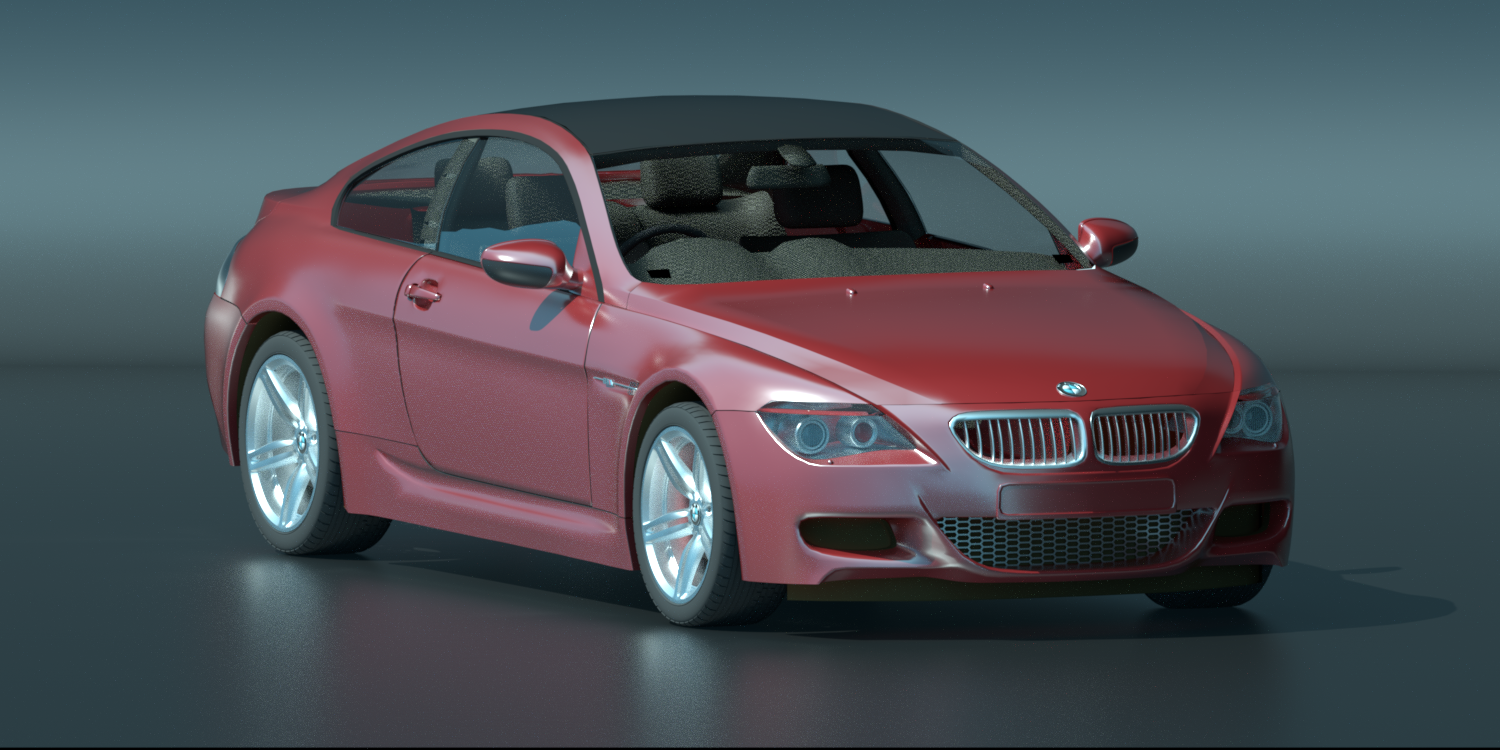
\includegraphics[width=\linewidth]{chap06/car-ortho.png}\label{fig:6.3.1}}\\
    \subfloat[透视]{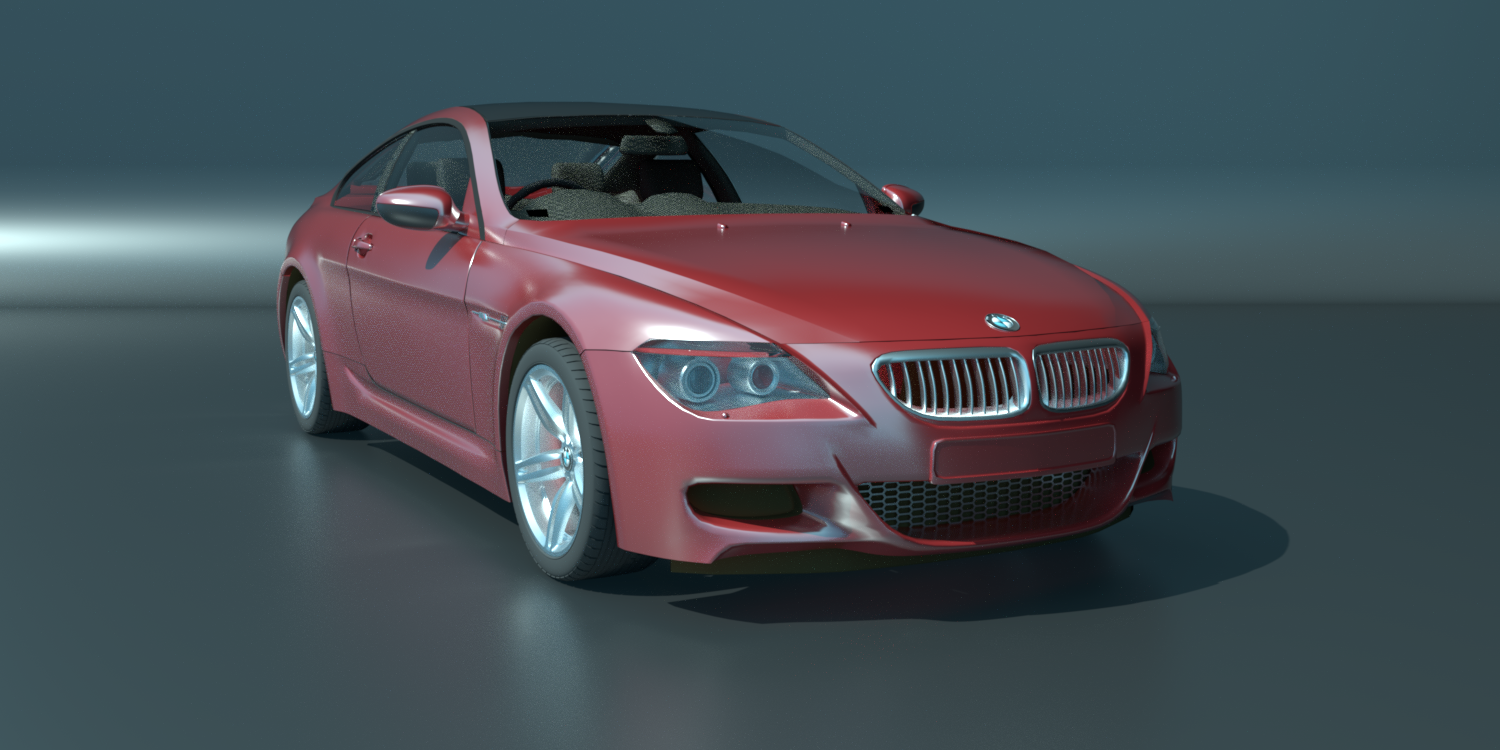
\includegraphics[width=\linewidth]{chap06/car-perspective.png}\label{fig:6.3.2}}
    \caption{用不同相机模型渲染的汽车模型。用(a)正交和(b)透视相机从同一视点渲染汽车。
        缺少前缩使得正交视角看起来深度更少,但它保留了平行线,是很有用的特性。}
    \label{fig:6.3}
\end{figure}

正交相机构造函数用稍后定义的函数\refvar{Orthographic}{()}生成正交变换矩阵。
\begin{lstlisting}
`\initcode{OrthographicCamera Public Methods}{=}`
`\refvar{OrthographicCamera}{}`(const `\refvar{AnimatedTransform}{}` &CameraToWorld,
        const `\refvar{Bounds2f}{}` &screenWindow, `\refvar{Float}{}` shutterOpen,
        `\refvar{Float}{}` shutterClose, `\refvar{Float}{}` lensRadius, `\refvar{Float}{}` focalDistance,
        `\refvar{Film}{}` *film, const `\refvar{Medium}{}` *medium)
    : `\refvar{ProjectiveCamera}{}`(CameraToWorld, `\refvar{Orthographic}{}`(0, 1),
                       screenWindow, shutterOpen, shutterClose,
                       lensRadius, focalDistance, film, medium) {
    `\refcode{Compute differential changes in origin for orthographic camera rays}{}`
}
\end{lstlisting}

正交视角变换保持$x$和$y$坐标不变但将近处平面的$z$值映射为0而远处平面的$z$值映射为1。
为此,场景先沿$z$轴平移使得近处平面对齐到$z=0$。
然后,场景按$z$缩放使得远处平面映射为$z=1$。
这两个变换合成得到整个变换。(对于像pbrt那样的光线追踪器,
我们想让近处平面位于0处,这样光线就会从穿过相机位置的平面上发出;
远处平面偏移量不是很重要。)
\begin{lstlisting}
`\refcode{Transform Method Definitions}{+=}\lastnext{TransformMethodDefinitions}`
`\refvar{Transform}{}` `\initvar{Orthographic}{}`(`\refvar{Float}{}` zNear, `\refvar{Float}{}` zFar) {
    return `\refvar{Scale}{}`(1, 1, 1 / (zFar - zNear)) *
           `\refvar{Translate}{}`(`\refvar{Vector3f}{}`(0, 0, -zNear));
}
\end{lstlisting}

幸亏正交投影很简单,在方法\refvar[OrthographicCamera::GenerateRayDifferential]{GenerateRayDifferential}{()}中
很容易直接计算$x$和$y$方向的差分射线。
差分射线的方向将和主射线一样(它们对于一个正交相机生成的所有光线都是这样),
且端点差异对于所有射线也会一样。
因此,这里的构造函数预先计算射线端点因胶片平面上在$x$和$y$方向移动单个像素而
在相机空间坐标中移动了多少。
\begin{lstlisting}
`\initcode{Compute differential changes in origin for orthographic camera rays}{=}`
`\refvar{dxCamera}{}` = `\refvar{RasterToCamera}{}`(`\refvar{Vector3f}{}`(1, 0, 0));
`\refvar{dyCamera}{}` = `\refvar{RasterToCamera}{}`(`\refvar{Vector3f}{}`(0, 1, 0));
\end{lstlisting}
\begin{lstlisting}
`\initcode{OrthographicCamera Private Data}{=}`
`\refvar{Vector3f}{}` `\initvar{dxCamera}{}`, `\initvar{dyCamera}{}`;
\end{lstlisting}

我们现在可以执行代码取栅格空间中的一个样本点并将其变为相机光线。
\reffig{6.4}总结了该过程。首先,栅格空间样本位置变换为相机空间的一点,
即给出近处平面上一点作为相机光线的端点。
因为相机空间观察方向沿$z$轴指出,相机空间光线方向为$(0,0,1)$。

\begin{figure}[htbp]
    \centering%LaTeX with PSTricks extensions
%%Creator: Inkscape 1.1.1 (3bf5ae0d25, 2021-09-20)
%%Please note this file requires PSTricks extensions
\psset{xunit=.5pt,yunit=.5pt,runit=.5pt}
\begin{pspicture}(595.2199707,244.36999512)
{
\newrgbcolor{curcolor}{0 0 0}
\pscustom[linewidth=1,linecolor=curcolor]
{
\newpath
\moveto(346.2,162.19999512)
\lineto(346.2,8.15999512)
\lineto(500.8,8.15999512)
}
}
{
\newrgbcolor{curcolor}{0 0 0}
\pscustom[linestyle=none,fillstyle=solid,fillcolor=curcolor]
{
\newpath
\moveto(340.7,157.28999512)
\lineto(346.2,161.54999512)
\lineto(351.71,157.28999512)
\lineto(346.2,170.29999512)
\closepath
}
}
{
\newrgbcolor{curcolor}{0.65098041 0.65098041 0.65098041}
\pscustom[linestyle=none,fillstyle=solid,fillcolor=curcolor]
{
\newpath
\moveto(341.9,158.83999512)
\lineto(346.2,168.98999512)
\lineto(346.2,162.17999512)
\closepath
}
}
{
\newrgbcolor{curcolor}{0.40000001 0.40000001 0.40000001}
\pscustom[linestyle=none,fillstyle=solid,fillcolor=curcolor]
{
\newpath
\moveto(350.5,158.83999512)
\lineto(346.2,168.98999512)
\lineto(346.2,162.17999512)
\closepath
}
}
{
\newrgbcolor{curcolor}{0 0 0}
\pscustom[linestyle=none,fillstyle=solid,fillcolor=curcolor]
{
\newpath
\moveto(495.89,2.65999512)
\lineto(500.15,8.15999512)
\lineto(495.89,13.66999512)
\lineto(508.9,8.15999512)
\closepath
}
}
{
\newrgbcolor{curcolor}{0.65098041 0.65098041 0.65098041}
\pscustom[linestyle=none,fillstyle=solid,fillcolor=curcolor]
{
\newpath
\moveto(497.45,3.85999512)
\lineto(507.59,8.15999512)
\lineto(500.78,8.15999512)
\closepath
}
}
{
\newrgbcolor{curcolor}{0.40000001 0.40000001 0.40000001}
\pscustom[linestyle=none,fillstyle=solid,fillcolor=curcolor]
{
\newpath
\moveto(497.45,12.45999512)
\lineto(507.59,8.15999512)
\lineto(500.78,8.15999512)
\closepath
}
}
{
\newrgbcolor{curcolor}{0 0 0}
\pscustom[linewidth=1,linecolor=curcolor]
{
\newpath
\moveto(559.29998779,221.28999519)
\lineto(346.20999146,8.20999146)
}
}
{
\newrgbcolor{curcolor}{0 0 0}
\pscustom[linestyle=none,fillstyle=solid,fillcolor=curcolor]
{
\newpath
\moveto(551.93,221.70999512)
\lineto(558.84,220.82999512)
\lineto(559.72,213.92999512)
\lineto(565.03,227.01999512)
\closepath
}
}
{
\newrgbcolor{curcolor}{0.65098041 0.65098041 0.65098041}
\pscustom[linestyle=none,fillstyle=solid,fillcolor=curcolor]
{
\newpath
\moveto(553.89,221.95999512)
\lineto(564.1,226.08999512)
\lineto(559.28,221.27999512)
\closepath
}
}
{
\newrgbcolor{curcolor}{0.40000001 0.40000001 0.40000001}
\pscustom[linestyle=none,fillstyle=solid,fillcolor=curcolor]
{
\newpath
\moveto(559.97,215.87999512)
\lineto(564.1,226.08999512)
\lineto(559.28,221.27999512)
\closepath
}
}
{
\newrgbcolor{curcolor}{0.60000002 0.60000002 0.60000002}
\pscustom[linestyle=none,fillstyle=solid,fillcolor=curcolor]
{
\newpath
\moveto(403.48001099,116.37999725)
\lineto(513.67001343,116.37999725)
\lineto(513.67001343,50.18000031)
\lineto(403.48001099,50.18000031)
\closepath
}
}
{
\newrgbcolor{curcolor}{0 0 0}
\pscustom[linewidth=1,linecolor=curcolor]
{
\newpath
\moveto(403.48001099,116.37999725)
\lineto(513.67001343,116.37999725)
\lineto(513.67001343,50.18000031)
\lineto(403.48001099,50.18000031)
\closepath
}
}
{
\newrgbcolor{curcolor}{0 0 0}
\pscustom[linewidth=1,linecolor=curcolor,linestyle=dashed,dash=2]
{
\newpath
\moveto(594.72,131.03999512)
\lineto(484.53,131.03999512)
\lineto(484.53,197.23999512)
}
}
{
\newrgbcolor{curcolor}{0 0 0}
\pscustom[linewidth=1,linecolor=curcolor]
{
\newpath
\moveto(484.53,197.23999512)
\lineto(594.72,197.23999512)
\lineto(594.72,131.03999512)
}
}
{
\newrgbcolor{curcolor}{0 0 0}
\pscustom[linewidth=1,linecolor=curcolor]
{
\newpath
\moveto(403.48001099,116.37999725)
\lineto(484.52999878,197.23999405)
}
}
{
\newrgbcolor{curcolor}{0.60000002 0.60000002 0.60000002}
\pscustom[linestyle=none,fillstyle=solid,fillcolor=curcolor]
{
\newpath
\moveto(513.67999268,116.37999725)
\lineto(594.7199707,197.23999405)
}
}
{
\newrgbcolor{curcolor}{0 0 0}
\pscustom[linewidth=1,linecolor=curcolor]
{
\newpath
\moveto(513.67999268,116.37999725)
\lineto(594.7199707,197.23999405)
}
}
{
\newrgbcolor{curcolor}{0.60000002 0.60000002 0.60000002}
\pscustom[linestyle=none,fillstyle=solid,fillcolor=curcolor]
{
\newpath
\moveto(594.7199707,131.03999329)
\lineto(513.67999268,50.17999268)
}
}
{
\newrgbcolor{curcolor}{0 0 0}
\pscustom[linewidth=1,linecolor=curcolor]
{
\newpath
\moveto(594.7199707,131.03999329)
\lineto(513.67999268,50.17999268)
}
}
{
\newrgbcolor{curcolor}{0.60000002 0.60000002 0.60000002}
\pscustom[linestyle=none,fillstyle=solid,fillcolor=curcolor]
{
\newpath
\moveto(484.52999878,131.03999329)
\lineto(403.48001099,50.17999268)
}
}
{
\newrgbcolor{curcolor}{0 0 0}
\pscustom[linewidth=1,linecolor=curcolor,linestyle=dashed,dash=2]
{
\newpath
\moveto(484.52999878,131.03999329)
\lineto(403.48001099,50.17999268)
}
}
{
\newrgbcolor{curcolor}{0.60000002 0.60000002 0.60000002}
\pscustom[linestyle=none,fillstyle=solid,fillcolor=curcolor]
{
\newpath
\moveto(17.02000046,171.70999146)
\lineto(182.35000229,171.70999146)
\lineto(182.35000229,72.38999176)
\lineto(17.02000046,72.38999176)
\closepath
}
}
{
\newrgbcolor{curcolor}{0 0 0}
\pscustom[linewidth=1,linecolor=curcolor]
{
\newpath
\moveto(17.02000046,171.70999146)
\lineto(182.35000229,171.70999146)
\lineto(182.35000229,72.38999176)
\lineto(17.02000046,72.38999176)
\closepath
}
}
{
\newrgbcolor{curcolor}{0 0 0}
\pscustom[linestyle=none,fillstyle=solid,fillcolor=curcolor]
{
\newpath
\moveto(108.08999634,92.86000061)
\curveto(108.08999634,94.86467594)(105.66643459,95.86825774)(104.2490869,94.45091005)
\curveto(102.83173921,93.03356236)(103.83532101,90.61000061)(105.83999634,90.61000061)
\curveto(107.84467166,90.61000061)(108.84825347,93.03356236)(107.43090578,94.45091005)
\curveto(106.01355808,95.86825774)(103.58999634,94.86467594)(103.58999634,92.86000061)
\curveto(103.58999634,90.85532528)(106.01355808,89.85174348)(107.43090578,91.26909117)
\curveto(108.84825347,92.68643886)(107.84467166,95.11000061)(105.83999634,95.11000061)
\curveto(103.83532101,95.11000061)(102.83173921,92.68643886)(104.2490869,91.26909117)
\curveto(105.66643459,89.85174348)(108.08999634,90.85532528)(108.08999634,92.86000061)
\closepath
}
}
{
\newrgbcolor{curcolor}{0 0 0}
\pscustom[linewidth=1,linecolor=curcolor]
{
\newpath
\moveto(108.08999634,92.86000061)
\curveto(108.08999634,94.86467594)(105.66643459,95.86825774)(104.2490869,94.45091005)
\curveto(102.83173921,93.03356236)(103.83532101,90.61000061)(105.83999634,90.61000061)
\curveto(107.84467166,90.61000061)(108.84825347,93.03356236)(107.43090578,94.45091005)
\curveto(106.01355808,95.86825774)(103.58999634,94.86467594)(103.58999634,92.86000061)
\curveto(103.58999634,90.85532528)(106.01355808,89.85174348)(107.43090578,91.26909117)
\curveto(108.84825347,92.68643886)(107.84467166,95.11000061)(105.83999634,95.11000061)
\curveto(103.83532101,95.11000061)(102.83173921,92.68643886)(104.2490869,91.26909117)
\curveto(105.66643459,89.85174348)(108.08999634,90.85532528)(108.08999634,92.86000061)
\closepath
}
}
{
\newrgbcolor{curcolor}{0 0 0}
\pscustom[linestyle=none,fillstyle=solid,fillcolor=curcolor]
{
\newpath
\moveto(184.25999451,72.69000244)
\curveto(184.25999451,74.69467777)(181.83643276,75.69825957)(180.41908507,74.28091188)
\curveto(179.00173738,72.86356419)(180.00531918,70.44000244)(182.00999451,70.44000244)
\curveto(184.01466983,70.44000244)(185.01825164,72.86356419)(183.60090394,74.28091188)
\curveto(182.18355625,75.69825957)(179.75999451,74.69467777)(179.75999451,72.69000244)
\curveto(179.75999451,70.68532712)(182.18355625,69.68174531)(183.60090394,71.099093)
\curveto(185.01825164,72.51644069)(184.01466983,74.94000244)(182.00999451,74.94000244)
\curveto(180.00531918,74.94000244)(179.00173738,72.51644069)(180.41908507,71.099093)
\curveto(181.83643276,69.68174531)(184.25999451,70.68532712)(184.25999451,72.69000244)
\closepath
}
}
{
\newrgbcolor{curcolor}{0 0 0}
\pscustom[linewidth=1,linecolor=curcolor]
{
\newpath
\moveto(184.25999451,72.69000244)
\curveto(184.25999451,74.69467777)(181.83643276,75.69825957)(180.41908507,74.28091188)
\curveto(179.00173738,72.86356419)(180.00531918,70.44000244)(182.00999451,70.44000244)
\curveto(184.01466983,70.44000244)(185.01825164,72.86356419)(183.60090394,74.28091188)
\curveto(182.18355625,75.69825957)(179.75999451,74.69467777)(179.75999451,72.69000244)
\curveto(179.75999451,70.68532712)(182.18355625,69.68174531)(183.60090394,71.099093)
\curveto(185.01825164,72.51644069)(184.01466983,74.94000244)(182.00999451,74.94000244)
\curveto(180.00531918,74.94000244)(179.00173738,72.51644069)(180.41908507,71.099093)
\curveto(181.83643276,69.68174531)(184.25999451,70.68532712)(184.25999451,72.69000244)
\closepath
}
}
{
\newrgbcolor{curcolor}{0 0 0}
\pscustom[linestyle=none,fillstyle=solid,fillcolor=curcolor]
{
\newpath
\moveto(19.76000023,171.18999481)
\curveto(19.76000023,173.19467014)(17.33643848,174.19825194)(15.91909079,172.78090425)
\curveto(14.5017431,171.36355656)(15.5053249,168.93999481)(17.51000023,168.93999481)
\curveto(19.51467556,168.93999481)(20.51825736,171.36355656)(19.10090967,172.78090425)
\curveto(17.68356198,174.19825194)(15.26000023,173.19467014)(15.26000023,171.18999481)
\curveto(15.26000023,169.18531949)(17.68356198,168.18173768)(19.10090967,169.59908537)
\curveto(20.51825736,171.01643307)(19.51467556,173.43999481)(17.51000023,173.43999481)
\curveto(15.5053249,173.43999481)(14.5017431,171.01643307)(15.91909079,169.59908537)
\curveto(17.33643848,168.18173768)(19.76000023,169.18531949)(19.76000023,171.18999481)
\closepath
}
}
{
\newrgbcolor{curcolor}{0 0 0}
\pscustom[linewidth=1,linecolor=curcolor]
{
\newpath
\moveto(19.76000023,171.18999481)
\curveto(19.76000023,173.19467014)(17.33643848,174.19825194)(15.91909079,172.78090425)
\curveto(14.5017431,171.36355656)(15.5053249,168.93999481)(17.51000023,168.93999481)
\curveto(19.51467556,168.93999481)(20.51825736,171.36355656)(19.10090967,172.78090425)
\curveto(17.68356198,174.19825194)(15.26000023,173.19467014)(15.26000023,171.18999481)
\curveto(15.26000023,169.18531949)(17.68356198,168.18173768)(19.10090967,169.59908537)
\curveto(20.51825736,171.01643307)(19.51467556,173.43999481)(17.51000023,173.43999481)
\curveto(15.5053249,173.43999481)(14.5017431,171.01643307)(15.91909079,169.59908537)
\curveto(17.33643848,168.18173768)(19.76000023,169.18531949)(19.76000023,171.18999481)
\closepath
}
}
{
\newrgbcolor{curcolor}{0 0 0}
\pscustom[linestyle=none,fillstyle=solid,fillcolor=curcolor]
{
\newpath
\moveto(462.26000977,62.36000061)
\curveto(462.26000977,64.36467594)(459.83644802,65.36825774)(458.41910033,63.95091005)
\curveto(457.00175264,62.53356236)(458.00533444,60.11000061)(460.01000977,60.11000061)
\curveto(462.01468509,60.11000061)(463.01826689,62.53356236)(461.6009192,63.95091005)
\curveto(460.18357151,65.36825774)(457.76000977,64.36467594)(457.76000977,62.36000061)
\curveto(457.76000977,60.35532528)(460.18357151,59.35174348)(461.6009192,60.76909117)
\curveto(463.01826689,62.18643886)(462.01468509,64.61000061)(460.01000977,64.61000061)
\curveto(458.00533444,64.61000061)(457.00175264,62.18643886)(458.41910033,60.76909117)
\curveto(459.83644802,59.35174348)(462.26000977,60.35532528)(462.26000977,62.36000061)
\closepath
}
}
{
\newrgbcolor{curcolor}{0 0 0}
\pscustom[linewidth=1,linecolor=curcolor]
{
\newpath
\moveto(462.26000977,62.36000061)
\curveto(462.26000977,64.36467594)(459.83644802,65.36825774)(458.41910033,63.95091005)
\curveto(457.00175264,62.53356236)(458.00533444,60.11000061)(460.01000977,60.11000061)
\curveto(462.01468509,60.11000061)(463.01826689,62.53356236)(461.6009192,63.95091005)
\curveto(460.18357151,65.36825774)(457.76000977,64.36467594)(457.76000977,62.36000061)
\curveto(457.76000977,60.35532528)(460.18357151,59.35174348)(461.6009192,60.76909117)
\curveto(463.01826689,62.18643886)(462.01468509,64.61000061)(460.01000977,64.61000061)
\curveto(458.00533444,64.61000061)(457.00175264,62.18643886)(458.41910033,60.76909117)
\curveto(459.83644802,59.35174348)(462.26000977,60.35532528)(462.26000977,62.36000061)
\closepath
}
}
{
\newrgbcolor{curcolor}{0 0 0}
\pscustom[linewidth=1,linecolor=curcolor]
{
\newpath
\moveto(459.57998657,62.69000244)
\lineto(502.64001465,105.75)
}
}
{
\newrgbcolor{curcolor}{0 0 0}
\pscustom[linestyle=none,fillstyle=solid,fillcolor=curcolor]
{
\newpath
\moveto(503.06,98.38999512)
\lineto(502.18,105.28999512)
\lineto(495.27,106.16999512)
\lineto(508.37,111.47999512)
\closepath
}
}
{
\newrgbcolor{curcolor}{0.65098041 0.65098041 0.65098041}
\pscustom[linestyle=none,fillstyle=solid,fillcolor=curcolor]
{
\newpath
\moveto(503.31,100.33999512)
\lineto(507.44,110.55999512)
\lineto(502.63,105.73999512)
\closepath
}
}
{
\newrgbcolor{curcolor}{0.40000001 0.40000001 0.40000001}
\pscustom[linestyle=none,fillstyle=solid,fillcolor=curcolor]
{
\newpath
\moveto(497.23,106.41999512)
\lineto(507.44,110.55999512)
\lineto(502.63,105.73999512)
\closepath
}
}
{
\newrgbcolor{curcolor}{0 0 0}
\pscustom[linewidth=1,linecolor=curcolor]
{
\newpath
\moveto(234.33999634,113.02999878)
\lineto(293.23999023,113.02999878)
}
}
{
\newrgbcolor{curcolor}{0 0 0}
\pscustom[linestyle=none,fillstyle=solid,fillcolor=curcolor]
{
\newpath
\moveto(288.33,107.51999512)
\lineto(292.59,113.02999512)
\lineto(288.33,118.52999512)
\lineto(301.34,113.02999512)
\closepath
}
}
{
\newrgbcolor{curcolor}{0.65098041 0.65098041 0.65098041}
\pscustom[linestyle=none,fillstyle=solid,fillcolor=curcolor]
{
\newpath
\moveto(289.89,108.71999512)
\lineto(300.03,113.02999512)
\lineto(293.22,113.02999512)
\closepath
}
}
{
\newrgbcolor{curcolor}{0.40000001 0.40000001 0.40000001}
\pscustom[linestyle=none,fillstyle=solid,fillcolor=curcolor]
{
\newpath
\moveto(289.89,117.31999512)
\lineto(300.03,113.02999512)
\lineto(293.22,113.02999512)
\closepath
}
}
{
\newrgbcolor{curcolor}{0 0 0}
\pscustom[linestyle=none,fillstyle=solid,fillcolor=curcolor]
{
\newpath
\moveto(350.5061361,187.41025924)
\curveto(350.5998861,187.69150924)(350.5998861,187.72275924)(350.5998861,187.87900924)
\curveto(350.5998861,188.22275924)(350.3186361,188.41025924)(350.0061361,188.41025924)
\curveto(349.8186361,188.41025924)(349.5061361,188.28525924)(349.3186361,188.00400924)
\curveto(349.2873861,187.87900924)(349.0998861,187.28525924)(349.0373861,186.91025924)
\curveto(348.8811361,186.41025924)(348.7561361,185.84775924)(348.6311361,185.31650924)
\lineto(347.7248861,181.72275924)
\curveto(347.6623861,181.44150924)(346.7873861,180.03525924)(345.4748861,180.03525924)
\curveto(344.4748861,180.03525924)(344.2561361,180.91025924)(344.2561361,181.66025924)
\curveto(344.2561361,182.56650924)(344.5998861,183.81650924)(345.2561361,185.56650924)
\curveto(345.5686361,186.37900924)(345.6623861,186.59775924)(345.6623861,187.00400924)
\curveto(345.6623861,187.87900924)(345.0373861,188.62900924)(344.0373861,188.62900924)
\curveto(342.1311361,188.62900924)(341.4123861,185.72275924)(341.4123861,185.56650924)
\curveto(341.4123861,185.34775924)(341.5998861,185.34775924)(341.6311361,185.34775924)
\curveto(341.8498861,185.34775924)(341.8498861,185.41025924)(341.9436361,185.72275924)
\curveto(342.5061361,187.59775924)(343.2873861,188.19150924)(343.9748861,188.19150924)
\curveto(344.1311361,188.19150924)(344.4748861,188.19150924)(344.4748861,187.56650924)
\curveto(344.4748861,187.06650924)(344.2561361,186.53525924)(344.1311361,186.16025924)
\curveto(343.3186361,184.03525924)(342.9748861,182.91025924)(342.9748861,181.97275924)
\curveto(342.9748861,180.19150924)(344.2248861,179.59775924)(345.4123861,179.59775924)
\curveto(346.1936361,179.59775924)(346.8498861,179.94150924)(347.4123861,180.50400924)
\curveto(347.1623861,179.47275924)(346.9123861,178.47275924)(346.1311361,177.41025924)
\curveto(345.5998861,176.75400924)(344.8498861,176.16025924)(343.9436361,176.16025924)
\curveto(343.6623861,176.16025924)(342.7561361,176.22275924)(342.4123861,177.00400924)
\curveto(342.7248861,177.00400924)(343.0061361,177.00400924)(343.2561361,177.25400924)
\curveto(343.4748861,177.41025924)(343.6623861,177.69150924)(343.6623861,178.06650924)
\curveto(343.6623861,178.69150924)(343.1311361,178.75400924)(342.9436361,178.75400924)
\curveto(342.4748861,178.75400924)(341.8186361,178.44150924)(341.8186361,177.47275924)
\curveto(341.8186361,176.47275924)(342.6936361,175.72275924)(343.9436361,175.72275924)
\curveto(345.9748861,175.72275924)(348.0373861,177.53525924)(348.5998861,179.78525924)
\closepath
\moveto(350.5061361,187.41025924)
}
}
{
\newrgbcolor{curcolor}{0 0 0}
\pscustom[linestyle=none,fillstyle=solid,fillcolor=curcolor]
{
\newpath
\moveto(527.3312561,9.56150024)
\curveto(527.4562561,10.06150024)(527.9250061,11.90525024)(529.3000061,11.90525024)
\curveto(529.3937561,11.90525024)(529.8937561,11.90525024)(530.3000061,11.65525024)
\curveto(529.7375061,11.53025024)(529.3625061,11.06150024)(529.3625061,10.56150024)
\curveto(529.3625061,10.24900024)(529.5812561,9.87400024)(530.1125061,9.87400024)
\curveto(530.5500061,9.87400024)(531.1750061,10.21775024)(531.1750061,11.03025024)
\curveto(531.1750061,12.06150024)(530.0187561,12.34275024)(529.3312561,12.34275024)
\curveto(528.1750061,12.34275024)(527.4875061,11.28025024)(527.2375061,10.84275024)
\curveto(526.7375061,12.15525024)(525.6750061,12.34275024)(525.0812561,12.34275024)
\curveto(523.0187561,12.34275024)(521.8625061,9.78025024)(521.8625061,9.28025024)
\curveto(521.8625061,9.06150024)(522.0812561,9.06150024)(522.1125061,9.06150024)
\curveto(522.2687561,9.06150024)(522.3312561,9.12400024)(522.3625061,9.28025024)
\curveto(523.0500061,11.40525024)(524.3625061,11.90525024)(525.0500061,11.90525024)
\curveto(525.4250061,11.90525024)(526.1125061,11.71775024)(526.1125061,10.56150024)
\curveto(526.1125061,9.93650024)(525.7687561,8.62400024)(525.0500061,5.81150024)
\curveto(524.7375061,4.59275024)(524.0187561,3.74900024)(523.1437561,3.74900024)
\curveto(523.0187561,3.74900024)(522.5812561,3.74900024)(522.1437561,3.99900024)
\curveto(522.6437561,4.12400024)(523.0812561,4.53025024)(523.0812561,5.09275024)
\curveto(523.0812561,5.62400024)(522.6437561,5.78025024)(522.3625061,5.78025024)
\curveto(521.7375061,5.78025024)(521.2687561,5.28025024)(521.2687561,4.62400024)
\curveto(521.2687561,3.71775024)(522.2375061,3.31150024)(523.1125061,3.31150024)
\curveto(524.4562561,3.31150024)(525.1750061,4.71775024)(525.2062561,4.81150024)
\curveto(525.4562561,4.09275024)(526.1750061,3.31150024)(527.3625061,3.31150024)
\curveto(529.4250061,3.31150024)(530.5500061,5.87400024)(530.5500061,6.37400024)
\curveto(530.5500061,6.59275024)(530.3937561,6.59275024)(530.3312561,6.59275024)
\curveto(530.1437561,6.59275024)(530.1125061,6.49900024)(530.0500061,6.37400024)
\curveto(529.3937561,4.21775024)(528.0500061,3.74900024)(527.4250061,3.74900024)
\curveto(526.6437561,3.74900024)(526.3312561,4.37400024)(526.3312561,5.06150024)
\curveto(526.3312561,5.49900024)(526.4250061,5.93650024)(526.6437561,6.81150024)
\closepath
\moveto(527.3312561,9.56150024)
}
}
{
\newrgbcolor{curcolor}{0 0 0}
\pscustom[linestyle=none,fillstyle=solid,fillcolor=curcolor]
{
\newpath
\moveto(572.0035161,229.26960024)
\curveto(573.0660161,230.42585024)(573.6597661,230.92585024)(574.3785161,231.55085024)
\curveto(574.3785161,231.55085024)(575.5972661,232.61335024)(576.3160161,233.33210024)
\curveto(578.2222661,235.17585024)(578.6597661,236.14460024)(578.6597661,236.23835024)
\curveto(578.6597661,236.42585024)(578.4722661,236.42585024)(578.4410161,236.42585024)
\curveto(578.2847661,236.42585024)(578.2535161,236.39460024)(578.1285161,236.20710024)
\curveto(577.5347661,235.23835024)(577.1285161,234.92585024)(576.6597661,234.92585024)
\curveto(576.1597661,234.92585024)(575.9410161,235.23835024)(575.6285161,235.58210024)
\curveto(575.2535161,236.01960024)(574.9097661,236.42585024)(574.2535161,236.42585024)
\curveto(572.7535161,236.42585024)(571.8472661,234.58210024)(571.8472661,234.14460024)
\curveto(571.8472661,234.05085024)(571.9097661,233.92585024)(572.0660161,233.92585024)
\curveto(572.2535161,233.92585024)(572.2847661,234.01960024)(572.3472661,234.14460024)
\curveto(572.7222661,235.08210024)(573.8785161,235.08210024)(574.0347661,235.08210024)
\curveto(574.4410161,235.08210024)(574.8160161,234.95710024)(575.2847661,234.80085024)
\curveto(576.0972661,234.48835024)(576.3160161,234.48835024)(576.8160161,234.48835024)
\curveto(576.0972661,233.64460024)(574.4410161,232.20710024)(574.0660161,231.89460024)
\lineto(572.2535161,230.20710024)
\curveto(570.9097661,228.86335024)(570.1910161,227.73835024)(570.1910161,227.58210024)
\curveto(570.1910161,227.39460024)(570.4097661,227.39460024)(570.4410161,227.39460024)
\curveto(570.5972661,227.39460024)(570.6285161,227.42585024)(570.7535161,227.64460024)
\curveto(571.2222661,228.36335024)(571.8160161,228.89460024)(572.4722661,228.89460024)
\curveto(572.9097661,228.89460024)(573.1285161,228.70710024)(573.6285161,228.14460024)
\curveto(573.9410161,227.70710024)(574.3160161,227.39460024)(574.8785161,227.39460024)
\curveto(576.8785161,227.39460024)(578.0347661,229.92585024)(578.0347661,230.45710024)
\curveto(578.0347661,230.55085024)(577.9410161,230.67585024)(577.7847661,230.67585024)
\curveto(577.5972661,230.67585024)(577.5660161,230.55085024)(577.5035161,230.39460024)
\curveto(577.0347661,229.11335024)(575.7535161,228.73835024)(575.0972661,228.73835024)
\curveto(574.7222661,228.73835024)(574.3472661,228.86335024)(573.9410161,228.98835024)
\curveto(573.2535161,229.23835024)(572.9410161,229.33210024)(572.5347661,229.33210024)
\curveto(572.5035161,229.33210024)(572.1910161,229.33210024)(572.0035161,229.26960024)
\closepath
\moveto(572.0035161,229.26960024)
}
}
{
\newrgbcolor{curcolor}{0 0 0}
\pscustom[linestyle=none,fillstyle=solid,fillcolor=curcolor]
{
\newpath
\moveto(8.3535661,176.03103024)
\curveto(8.3535661,176.09353024)(8.3535661,176.12478024)(8.0098161,176.46853024)
\curveto(5.5410661,178.96853024)(4.8848161,182.74978024)(4.8848161,185.81228024)
\curveto(4.8848161,189.28103024)(5.6348161,192.74978024)(8.1035661,195.21853024)
\curveto(8.3535661,195.46853024)(8.3535661,195.49978024)(8.3535661,195.56228024)
\curveto(8.3535661,195.71853024)(8.2910661,195.78103024)(8.1660661,195.78103024)
\curveto(7.9473161,195.78103024)(6.1660661,194.40603024)(4.9785661,191.87478024)
\curveto(3.9785661,189.68728024)(3.7285661,187.46853024)(3.7285661,185.81228024)
\curveto(3.7285661,184.24978024)(3.9473161,181.84353024)(5.0410661,179.56228024)
\curveto(6.2598161,177.12478024)(7.9473161,175.81228024)(8.1660661,175.81228024)
\curveto(8.2910661,175.81228024)(8.3535661,175.87478024)(8.3535661,176.03103024)
\closepath
\moveto(8.3535661,176.03103024)
}
}
{
\newrgbcolor{curcolor}{0 0 0}
\pscustom[linestyle=none,fillstyle=solid,fillcolor=curcolor]
{
\newpath
\moveto(18.66496747,187.18728024)
\curveto(18.66496747,188.78103024)(18.57121747,190.37478024)(17.88371747,191.84353024)
\curveto(16.97746747,193.78103024)(15.32121747,194.09353024)(14.50871747,194.09353024)
\curveto(13.28996747,194.09353024)(11.85246747,193.56228024)(11.00871747,191.71853024)
\curveto(10.38371747,190.34353024)(10.28996747,188.78103024)(10.28996747,187.18728024)
\curveto(10.28996747,185.68728024)(10.35246747,183.90603024)(11.19621747,182.37478024)
\curveto(12.03996747,180.78103024)(13.50871747,180.37478024)(14.47746747,180.37478024)
\curveto(15.53996747,180.37478024)(17.07121747,180.78103024)(17.94621747,182.68728024)
\curveto(18.57121747,184.06228024)(18.66496747,185.62478024)(18.66496747,187.18728024)
\closepath
\moveto(14.47746747,180.81228024)
\curveto(13.69621747,180.81228024)(12.50871747,181.31228024)(12.16496747,183.21853024)
\curveto(11.94621747,184.40603024)(11.94621747,186.24978024)(11.94621747,187.43728024)
\curveto(11.94621747,188.71853024)(11.94621747,190.03103024)(12.10246747,191.09353024)
\curveto(12.47746747,193.46853024)(13.97746747,193.65603024)(14.47746747,193.65603024)
\curveto(15.13371747,193.65603024)(16.44621747,193.28103024)(16.82121747,191.31228024)
\curveto(17.03996747,190.18728024)(17.03996747,188.68728024)(17.03996747,187.43728024)
\curveto(17.03996747,185.93728024)(17.03996747,184.59353024)(16.82121747,183.31228024)
\curveto(16.50871747,181.40603024)(15.38371747,180.81228024)(14.47746747,180.81228024)
\closepath
\moveto(14.47746747,180.81228024)
}
}
{
\newrgbcolor{curcolor}{0 0 0}
\pscustom[linestyle=none,fillstyle=solid,fillcolor=curcolor]
{
\newpath
\moveto(23.53430646,180.84353024)
\curveto(23.53430646,182.15603024)(23.03430646,182.93728024)(22.25305646,182.93728024)
\curveto(21.59680646,182.93728024)(21.19055646,182.43728024)(21.19055646,181.87478024)
\curveto(21.19055646,181.34353024)(21.59680646,180.81228024)(22.25305646,180.81228024)
\curveto(22.47180646,180.81228024)(22.75305646,180.90603024)(22.94055646,181.06228024)
\curveto(23.00305646,181.12478024)(23.03430646,181.12478024)(23.03430646,181.12478024)
\curveto(23.06555646,181.12478024)(23.06555646,181.12478024)(23.06555646,180.84353024)
\curveto(23.06555646,179.34353024)(22.37805646,178.15603024)(21.72180646,177.49978024)
\curveto(21.50305646,177.28103024)(21.50305646,177.24978024)(21.50305646,177.18728024)
\curveto(21.50305646,177.03103024)(21.59680646,176.96853024)(21.69055646,176.96853024)
\curveto(21.90930646,176.96853024)(23.53430646,178.49978024)(23.53430646,180.84353024)
\closepath
\moveto(23.53430646,180.84353024)
}
}
{
\newrgbcolor{curcolor}{0 0 0}
\pscustom[linestyle=none,fillstyle=solid,fillcolor=curcolor]
{
\newpath
\moveto(37.48405927,187.18728024)
\curveto(37.48405927,188.78103024)(37.39030927,190.37478024)(36.70280927,191.84353024)
\curveto(35.79655927,193.78103024)(34.14030927,194.09353024)(33.32780927,194.09353024)
\curveto(32.10905927,194.09353024)(30.67155927,193.56228024)(29.82780927,191.71853024)
\curveto(29.20280927,190.34353024)(29.10905927,188.78103024)(29.10905927,187.18728024)
\curveto(29.10905927,185.68728024)(29.17155927,183.90603024)(30.01530927,182.37478024)
\curveto(30.85905927,180.78103024)(32.32780927,180.37478024)(33.29655927,180.37478024)
\curveto(34.35905927,180.37478024)(35.89030927,180.78103024)(36.76530927,182.68728024)
\curveto(37.39030927,184.06228024)(37.48405927,185.62478024)(37.48405927,187.18728024)
\closepath
\moveto(33.29655927,180.81228024)
\curveto(32.51530927,180.81228024)(31.32780927,181.31228024)(30.98405927,183.21853024)
\curveto(30.76530927,184.40603024)(30.76530927,186.24978024)(30.76530927,187.43728024)
\curveto(30.76530927,188.71853024)(30.76530927,190.03103024)(30.92155927,191.09353024)
\curveto(31.29655927,193.46853024)(32.79655927,193.65603024)(33.29655927,193.65603024)
\curveto(33.95280927,193.65603024)(35.26530927,193.28103024)(35.64030927,191.31228024)
\curveto(35.85905927,190.18728024)(35.85905927,188.68728024)(35.85905927,187.43728024)
\curveto(35.85905927,185.93728024)(35.85905927,184.59353024)(35.64030927,183.31228024)
\curveto(35.32780927,181.40603024)(34.20280927,180.81228024)(33.29655927,180.81228024)
\closepath
\moveto(33.29655927,180.81228024)
}
}
{
\newrgbcolor{curcolor}{0 0 0}
\pscustom[linestyle=none,fillstyle=solid,fillcolor=curcolor]
{
\newpath
\moveto(44.04040998,185.81228024)
\curveto(44.04040998,187.34353024)(43.82165998,189.74978024)(42.72790998,192.03103024)
\curveto(41.54040998,194.46853024)(39.82165998,195.78103024)(39.63415998,195.78103024)
\curveto(39.50915998,195.78103024)(39.41540998,195.68728024)(39.41540998,195.56228024)
\curveto(39.41540998,195.49978024)(39.41540998,195.46853024)(39.79040998,195.09353024)
\curveto(41.75915998,193.12478024)(42.88415998,189.96853024)(42.88415998,185.81228024)
\curveto(42.88415998,182.37478024)(42.16540998,178.87478024)(39.69665998,176.37478024)
\curveto(39.41540998,176.12478024)(39.41540998,176.09353024)(39.41540998,176.03103024)
\curveto(39.41540998,175.90603024)(39.50915998,175.81228024)(39.63415998,175.81228024)
\curveto(39.82165998,175.81228024)(41.63415998,177.18728024)(42.79040998,179.71853024)
\curveto(43.82165998,181.90603024)(44.04040998,184.12478024)(44.04040998,185.81228024)
\closepath
\moveto(44.04040998,185.81228024)
}
}
{
\newrgbcolor{curcolor}{0 0 0}
\pscustom[linestyle=none,fillstyle=solid,fillcolor=curcolor]
{
\newpath
\moveto(142.2842861,45.08760624)
\curveto(142.2842861,45.15010624)(142.2842861,45.18135624)(141.9405361,45.52510624)
\curveto(139.4717861,48.02510624)(138.8155361,51.80635624)(138.8155361,54.86885624)
\curveto(138.8155361,58.33760624)(139.5655361,61.80635624)(142.0342861,64.27510624)
\curveto(142.2842861,64.52510624)(142.2842861,64.55635624)(142.2842861,64.61885624)
\curveto(142.2842861,64.77510624)(142.2217861,64.83760624)(142.0967861,64.83760624)
\curveto(141.8780361,64.83760624)(140.0967861,63.46260624)(138.9092861,60.93135624)
\curveto(137.9092861,58.74385624)(137.6592861,56.52510624)(137.6592861,54.86885624)
\curveto(137.6592861,53.30635624)(137.8780361,50.90010624)(138.9717861,48.61885624)
\curveto(140.1905361,46.18135624)(141.8780361,44.86885624)(142.0967861,44.86885624)
\curveto(142.2217861,44.86885624)(142.2842861,44.93135624)(142.2842861,45.08760624)
\closepath
\moveto(142.2842861,45.08760624)
}
}
{
\newrgbcolor{curcolor}{0 0 0}
\pscustom[linestyle=none,fillstyle=solid,fillcolor=curcolor]
{
\newpath
\moveto(149.15818747,54.55635624)
\curveto(149.75193747,55.30635624)(150.50193747,56.27510624)(151.00193747,56.80635624)
\curveto(151.62693747,57.52510624)(152.43943747,57.83760624)(153.37693747,57.83760624)
\lineto(153.37693747,58.46260624)
\curveto(152.84568747,58.43135624)(152.25193747,58.40010624)(151.72068747,58.40010624)
\curveto(151.12693747,58.40010624)(150.06443747,58.43135624)(149.81443747,58.46260624)
\lineto(149.81443747,57.83760624)
\curveto(150.25193747,57.80635624)(150.40818747,57.55635624)(150.40818747,57.21260624)
\curveto(150.40818747,56.90010624)(150.18943747,56.65010624)(150.09568747,56.52510624)
\lineto(148.87693747,54.96260624)
\lineto(147.31443747,56.99385624)
\curveto(147.12693747,57.18135624)(147.12693747,57.21260624)(147.12693747,57.33760624)
\curveto(147.12693747,57.65010624)(147.43943747,57.83760624)(147.81443747,57.83760624)
\lineto(147.81443747,58.46260624)
\curveto(147.31443747,58.43135624)(146.00193747,58.40010624)(145.65818747,58.40010624)
\curveto(145.25193747,58.40010624)(144.31443747,58.43135624)(143.78318747,58.46260624)
\lineto(143.78318747,57.83760624)
\curveto(145.18943747,57.83760624)(145.18943747,57.83760624)(146.12693747,56.61885624)
\lineto(148.09568747,54.05635624)
\lineto(146.22068747,51.68135624)
\curveto(145.28318747,50.52510624)(144.09568747,50.49385624)(143.68943747,50.49385624)
\lineto(143.68943747,49.86885624)
\curveto(144.18943747,49.90010624)(144.81443747,49.93135624)(145.34568747,49.93135624)
\curveto(145.90818747,49.93135624)(146.75193747,49.90010624)(147.22068747,49.86885624)
\lineto(147.22068747,50.49385624)
\curveto(146.78318747,50.55635624)(146.65818747,50.80635624)(146.65818747,51.11885624)
\curveto(146.65818747,51.55635624)(147.22068747,52.21260624)(148.43943747,53.65010624)
\lineto(149.97068747,51.65010624)
\curveto(150.12693747,51.43135624)(150.37693747,51.11885624)(150.37693747,50.99385624)
\curveto(150.37693747,50.80635624)(150.18943747,50.49385624)(149.65818747,50.49385624)
\lineto(149.65818747,49.86885624)
\curveto(150.25193747,49.90010624)(151.37693747,49.93135624)(151.81443747,49.93135624)
\curveto(152.34568747,49.93135624)(153.12693747,49.90010624)(153.72068747,49.86885624)
\lineto(153.72068747,50.49385624)
\curveto(152.65818747,50.49385624)(152.28318747,50.52510624)(151.84568747,51.11885624)
\closepath
\moveto(149.15818747,54.55635624)
}
}
{
\newrgbcolor{curcolor}{0 0 0}
\pscustom[linestyle=none,fillstyle=solid,fillcolor=curcolor]
{
\newpath
\moveto(158.42471274,56.90010624)
\lineto(158.42471274,62.05635624)
\curveto(158.42471274,62.52510624)(158.42471274,62.77510624)(158.86221274,62.83760624)
\curveto(159.04971274,62.86885624)(159.64346274,62.86885624)(160.04971274,62.86885624)
\curveto(161.83096274,62.86885624)(164.04971274,62.77510624)(164.04971274,59.90010624)
\curveto(164.04971274,58.52510624)(163.58096274,56.90010624)(160.64346274,56.90010624)
\closepath
\moveto(162.64346274,56.65010624)
\curveto(164.54971274,57.11885624)(166.11221274,58.33760624)(166.11221274,59.90010624)
\curveto(166.11221274,61.80635624)(163.83096274,63.49385624)(160.92471274,63.49385624)
\lineto(154.64346274,63.49385624)
\lineto(154.64346274,62.86885624)
\lineto(155.14346274,62.86885624)
\curveto(156.67471274,62.86885624)(156.70596274,62.65010624)(156.70596274,61.93135624)
\lineto(156.70596274,51.43135624)
\curveto(156.70596274,50.71260624)(156.67471274,50.49385624)(155.14346274,50.49385624)
\lineto(154.64346274,50.49385624)
\lineto(154.64346274,49.86885624)
\curveto(155.36221274,49.93135624)(156.79971274,49.93135624)(157.54971274,49.93135624)
\curveto(158.33096274,49.93135624)(159.76846274,49.93135624)(160.48721274,49.86885624)
\lineto(160.48721274,50.49385624)
\lineto(159.98721274,50.49385624)
\curveto(158.45596274,50.49385624)(158.42471274,50.71260624)(158.42471274,51.43135624)
\lineto(158.42471274,56.46260624)
\lineto(160.70596274,56.46260624)
\curveto(161.01846274,56.46260624)(161.86221274,56.46260624)(162.58096274,55.77510624)
\curveto(163.33096274,55.08760624)(163.33096274,54.46260624)(163.33096274,53.11885624)
\curveto(163.33096274,51.83760624)(163.33096274,51.02510624)(164.14346274,50.27510624)
\curveto(164.95596274,49.55635624)(166.04971274,49.43135624)(166.64346274,49.43135624)
\curveto(168.20596274,49.43135624)(168.54971274,51.05635624)(168.54971274,51.61885624)
\curveto(168.54971274,51.74385624)(168.54971274,51.96260624)(168.29971274,51.96260624)
\curveto(168.08096274,51.96260624)(168.08096274,51.77510624)(168.04971274,51.65010624)
\curveto(167.92471274,50.21260624)(167.23721274,49.86885624)(166.73721274,49.86885624)
\curveto(165.76846274,49.86885624)(165.61221274,50.90010624)(165.33096274,52.74385624)
\lineto(165.04971274,54.33760624)
\curveto(164.70596274,55.61885624)(163.73721274,56.27510624)(162.64346274,56.65010624)
\closepath
\moveto(162.64346274,56.65010624)
}
}
{
\newrgbcolor{curcolor}{0 0 0}
\pscustom[linestyle=none,fillstyle=solid,fillcolor=curcolor]
{
\newpath
\moveto(170.84164389,54.90010624)
\curveto(170.96664389,57.86885624)(172.65414389,58.36885624)(173.34164389,58.36885624)
\curveto(175.37289389,58.36885624)(175.59164389,55.68135624)(175.59164389,54.90010624)
\closepath
\moveto(170.84164389,54.46260624)
\lineto(176.40414389,54.46260624)
\curveto(176.84164389,54.46260624)(176.90414389,54.46260624)(176.90414389,54.90010624)
\curveto(176.90414389,56.86885624)(175.81039389,58.80635624)(173.34164389,58.80635624)
\curveto(171.02914389,58.80635624)(169.18539389,56.74385624)(169.18539389,54.24385624)
\curveto(169.18539389,51.58760624)(171.27914389,49.65010624)(173.56039389,49.65010624)
\curveto(175.99789389,49.65010624)(176.90414389,51.86885624)(176.90414389,52.24385624)
\curveto(176.90414389,52.43135624)(176.74789389,52.49385624)(176.62289389,52.49385624)
\curveto(176.46664389,52.49385624)(176.40414389,52.36885624)(176.37289389,52.21260624)
\curveto(175.68539389,50.15010624)(173.87289389,50.15010624)(173.68539389,50.15010624)
\curveto(172.68539389,50.15010624)(171.90414389,50.74385624)(171.43539389,51.49385624)
\curveto(170.84164389,52.43135624)(170.84164389,53.74385624)(170.84164389,54.46260624)
\closepath
\moveto(170.84164389,54.46260624)
}
}
{
\newrgbcolor{curcolor}{0 0 0}
\pscustom[linestyle=none,fillstyle=solid,fillcolor=curcolor]
{
\newpath
\moveto(181.633926,53.74385624)
\curveto(182.071426,53.65010624)(183.696426,53.33760624)(183.696426,51.90010624)
\curveto(183.696426,50.90010624)(183.008926,50.08760624)(181.446426,50.08760624)
\curveto(179.758926,50.08760624)(179.040176,51.21260624)(178.665176,52.93135624)
\curveto(178.602676,53.18135624)(178.602676,53.24385624)(178.383926,53.24385624)
\curveto(178.133926,53.24385624)(178.133926,53.11885624)(178.133926,52.77510624)
\lineto(178.133926,50.11885624)
\curveto(178.133926,49.77510624)(178.133926,49.65010624)(178.352676,49.65010624)
\curveto(178.446426,49.65010624)(178.477676,49.68135624)(178.852676,50.05635624)
\curveto(178.883926,50.08760624)(178.883926,50.11885624)(179.258926,50.49385624)
\curveto(180.133926,49.68135624)(181.040176,49.65010624)(181.446426,49.65010624)
\curveto(183.727676,49.65010624)(184.665176,50.99385624)(184.665176,52.43135624)
\curveto(184.665176,53.46260624)(184.071426,54.08760624)(183.821426,54.30635624)
\curveto(183.165176,54.96260624)(182.383926,55.11885624)(181.540176,55.27510624)
\curveto(180.415176,55.49385624)(179.102676,55.74385624)(179.102676,56.90010624)
\curveto(179.102676,57.61885624)(179.602676,58.43135624)(181.321426,58.43135624)
\curveto(183.508926,58.43135624)(183.633926,56.61885624)(183.665176,56.02510624)
\curveto(183.665176,55.83760624)(183.852676,55.83760624)(183.883926,55.83760624)
\curveto(184.165176,55.83760624)(184.165176,55.93135624)(184.165176,56.30635624)
\lineto(184.165176,58.33760624)
\curveto(184.165176,58.65010624)(184.165176,58.80635624)(183.946426,58.80635624)
\curveto(183.852676,58.80635624)(183.790176,58.80635624)(183.540176,58.55635624)
\curveto(183.477676,58.49385624)(183.290176,58.30635624)(183.196426,58.24385624)
\curveto(182.446426,58.80635624)(181.633926,58.80635624)(181.321426,58.80635624)
\curveto(178.883926,58.80635624)(178.133926,57.46260624)(178.133926,56.33760624)
\curveto(178.133926,55.65010624)(178.446426,55.08760624)(178.977676,54.65010624)
\curveto(179.633926,54.15010624)(180.196426,54.02510624)(181.633926,53.74385624)
\closepath
\moveto(181.633926,53.74385624)
}
}
{
\newrgbcolor{curcolor}{0 0 0}
\pscustom[linestyle=none,fillstyle=solid,fillcolor=curcolor]
{
\newpath
\moveto(189.4010311,49.90010624)
\curveto(189.4010311,51.21260624)(188.9010311,51.99385624)(188.1197811,51.99385624)
\curveto(187.4635311,51.99385624)(187.0572811,51.49385624)(187.0572811,50.93135624)
\curveto(187.0572811,50.40010624)(187.4635311,49.86885624)(188.1197811,49.86885624)
\curveto(188.3385311,49.86885624)(188.6197811,49.96260624)(188.8072811,50.11885624)
\curveto(188.8697811,50.18135624)(188.9010311,50.18135624)(188.9010311,50.18135624)
\curveto(188.9322811,50.18135624)(188.9322811,50.18135624)(188.9322811,49.90010624)
\curveto(188.9322811,48.40010624)(188.2447811,47.21260624)(187.5885311,46.55635624)
\curveto(187.3697811,46.33760624)(187.3697811,46.30635624)(187.3697811,46.24385624)
\curveto(187.3697811,46.08760624)(187.4635311,46.02510624)(187.5572811,46.02510624)
\curveto(187.7760311,46.02510624)(189.4010311,47.55635624)(189.4010311,49.90010624)
\closepath
\moveto(189.4010311,49.90010624)
}
}
{
\newrgbcolor{curcolor}{0 0 0}
\pscustom[linestyle=none,fillstyle=solid,fillcolor=curcolor]
{
\newpath
\moveto(202.47578391,56.55635624)
\curveto(202.97578391,57.83760624)(204.00703391,57.83760624)(204.31953391,57.83760624)
\lineto(204.31953391,58.46260624)
\curveto(203.85078391,58.43135624)(203.28828391,58.40010624)(202.81953391,58.40010624)
\curveto(202.47578391,58.40010624)(201.53828391,58.43135624)(201.10078391,58.46260624)
\lineto(201.10078391,57.83760624)
\curveto(201.72578391,57.83760624)(202.03828391,57.49385624)(202.03828391,56.99385624)
\curveto(202.03828391,56.77510624)(202.00703391,56.74385624)(201.91328391,56.49385624)
\lineto(199.88203391,51.61885624)
\lineto(197.69453391,56.96260624)
\curveto(197.60078391,57.18135624)(197.56953391,57.24385624)(197.56953391,57.33760624)
\curveto(197.56953391,57.83760624)(198.28828391,57.83760624)(198.69453391,57.83760624)
\lineto(198.69453391,58.46260624)
\curveto(198.16328391,58.43135624)(196.85078391,58.40010624)(196.50703391,58.40010624)
\curveto(195.97578391,58.40010624)(195.16328391,58.43135624)(194.56953391,58.46260624)
\lineto(194.56953391,57.83760624)
\curveto(195.53828391,57.83760624)(195.91328391,57.83760624)(196.19453391,57.15010624)
\lineto(199.19453391,49.86885624)
\curveto(199.06953391,49.61885624)(198.78828391,48.96260624)(198.69453391,48.68135624)
\curveto(198.25703391,47.58760624)(197.69453391,46.21260624)(196.41328391,46.21260624)
\curveto(196.31953391,46.21260624)(195.85078391,46.21260624)(195.47578391,46.58760624)
\curveto(196.10078391,46.65010624)(196.25703391,47.08760624)(196.25703391,47.43135624)
\curveto(196.25703391,47.93135624)(195.88203391,48.24385624)(195.41328391,48.24385624)
\curveto(195.00703391,48.24385624)(194.56953391,47.99385624)(194.56953391,47.40010624)
\curveto(194.56953391,46.49385624)(195.41328391,45.77510624)(196.41328391,45.77510624)
\curveto(197.66328391,45.77510624)(198.47578391,46.93135624)(198.94453391,48.05635624)
\closepath
\moveto(202.47578391,56.55635624)
}
}
{
\newrgbcolor{curcolor}{0 0 0}
\pscustom[linestyle=none,fillstyle=solid,fillcolor=curcolor]
{
\newpath
\moveto(209.17979392,56.90010624)
\lineto(209.17979392,62.05635624)
\curveto(209.17979392,62.52510624)(209.17979392,62.77510624)(209.61729392,62.83760624)
\curveto(209.80479392,62.86885624)(210.39854392,62.86885624)(210.80479392,62.86885624)
\curveto(212.58604392,62.86885624)(214.80479392,62.77510624)(214.80479392,59.90010624)
\curveto(214.80479392,58.52510624)(214.33604392,56.90010624)(211.39854392,56.90010624)
\closepath
\moveto(213.39854392,56.65010624)
\curveto(215.30479392,57.11885624)(216.86729392,58.33760624)(216.86729392,59.90010624)
\curveto(216.86729392,61.80635624)(214.58604392,63.49385624)(211.67979392,63.49385624)
\lineto(205.39854392,63.49385624)
\lineto(205.39854392,62.86885624)
\lineto(205.89854392,62.86885624)
\curveto(207.42979392,62.86885624)(207.46104392,62.65010624)(207.46104392,61.93135624)
\lineto(207.46104392,51.43135624)
\curveto(207.46104392,50.71260624)(207.42979392,50.49385624)(205.89854392,50.49385624)
\lineto(205.39854392,50.49385624)
\lineto(205.39854392,49.86885624)
\curveto(206.11729392,49.93135624)(207.55479392,49.93135624)(208.30479392,49.93135624)
\curveto(209.08604392,49.93135624)(210.52354392,49.93135624)(211.24229392,49.86885624)
\lineto(211.24229392,50.49385624)
\lineto(210.74229392,50.49385624)
\curveto(209.21104392,50.49385624)(209.17979392,50.71260624)(209.17979392,51.43135624)
\lineto(209.17979392,56.46260624)
\lineto(211.46104392,56.46260624)
\curveto(211.77354392,56.46260624)(212.61729392,56.46260624)(213.33604392,55.77510624)
\curveto(214.08604392,55.08760624)(214.08604392,54.46260624)(214.08604392,53.11885624)
\curveto(214.08604392,51.83760624)(214.08604392,51.02510624)(214.89854392,50.27510624)
\curveto(215.71104392,49.55635624)(216.80479392,49.43135624)(217.39854392,49.43135624)
\curveto(218.96104392,49.43135624)(219.30479392,51.05635624)(219.30479392,51.61885624)
\curveto(219.30479392,51.74385624)(219.30479392,51.96260624)(219.05479392,51.96260624)
\curveto(218.83604392,51.96260624)(218.83604392,51.77510624)(218.80479392,51.65010624)
\curveto(218.67979392,50.21260624)(217.99229392,49.86885624)(217.49229392,49.86885624)
\curveto(216.52354392,49.86885624)(216.36729392,50.90010624)(216.08604392,52.74385624)
\lineto(215.80479392,54.33760624)
\curveto(215.46104392,55.61885624)(214.49229392,56.27510624)(213.39854392,56.65010624)
\closepath
\moveto(213.39854392,56.65010624)
}
}
{
\newrgbcolor{curcolor}{0 0 0}
\pscustom[linestyle=none,fillstyle=solid,fillcolor=curcolor]
{
\newpath
\moveto(221.59672507,54.90010624)
\curveto(221.72172507,57.86885624)(223.40922507,58.36885624)(224.09672507,58.36885624)
\curveto(226.12797507,58.36885624)(226.34672507,55.68135624)(226.34672507,54.90010624)
\closepath
\moveto(221.59672507,54.46260624)
\lineto(227.15922507,54.46260624)
\curveto(227.59672507,54.46260624)(227.65922507,54.46260624)(227.65922507,54.90010624)
\curveto(227.65922507,56.86885624)(226.56547507,58.80635624)(224.09672507,58.80635624)
\curveto(221.78422507,58.80635624)(219.94047507,56.74385624)(219.94047507,54.24385624)
\curveto(219.94047507,51.58760624)(222.03422507,49.65010624)(224.31547507,49.65010624)
\curveto(226.75297507,49.65010624)(227.65922507,51.86885624)(227.65922507,52.24385624)
\curveto(227.65922507,52.43135624)(227.50297507,52.49385624)(227.37797507,52.49385624)
\curveto(227.22172507,52.49385624)(227.15922507,52.36885624)(227.12797507,52.21260624)
\curveto(226.44047507,50.15010624)(224.62797507,50.15010624)(224.44047507,50.15010624)
\curveto(223.44047507,50.15010624)(222.65922507,50.74385624)(222.19047507,51.49385624)
\curveto(221.59672507,52.43135624)(221.59672507,53.74385624)(221.59672507,54.46260624)
\closepath
\moveto(221.59672507,54.46260624)
}
}
{
\newrgbcolor{curcolor}{0 0 0}
\pscustom[linestyle=none,fillstyle=solid,fillcolor=curcolor]
{
\newpath
\moveto(232.38899191,53.74385624)
\curveto(232.82649191,53.65010624)(234.45149191,53.33760624)(234.45149191,51.90010624)
\curveto(234.45149191,50.90010624)(233.76399191,50.08760624)(232.20149191,50.08760624)
\curveto(230.51399191,50.08760624)(229.79524191,51.21260624)(229.42024191,52.93135624)
\curveto(229.35774191,53.18135624)(229.35774191,53.24385624)(229.13899191,53.24385624)
\curveto(228.88899191,53.24385624)(228.88899191,53.11885624)(228.88899191,52.77510624)
\lineto(228.88899191,50.11885624)
\curveto(228.88899191,49.77510624)(228.88899191,49.65010624)(229.10774191,49.65010624)
\curveto(229.20149191,49.65010624)(229.23274191,49.68135624)(229.60774191,50.05635624)
\curveto(229.63899191,50.08760624)(229.63899191,50.11885624)(230.01399191,50.49385624)
\curveto(230.88899191,49.68135624)(231.79524191,49.65010624)(232.20149191,49.65010624)
\curveto(234.48274191,49.65010624)(235.42024191,50.99385624)(235.42024191,52.43135624)
\curveto(235.42024191,53.46260624)(234.82649191,54.08760624)(234.57649191,54.30635624)
\curveto(233.92024191,54.96260624)(233.13899191,55.11885624)(232.29524191,55.27510624)
\curveto(231.17024191,55.49385624)(229.85774191,55.74385624)(229.85774191,56.90010624)
\curveto(229.85774191,57.61885624)(230.35774191,58.43135624)(232.07649191,58.43135624)
\curveto(234.26399191,58.43135624)(234.38899191,56.61885624)(234.42024191,56.02510624)
\curveto(234.42024191,55.83760624)(234.60774191,55.83760624)(234.63899191,55.83760624)
\curveto(234.92024191,55.83760624)(234.92024191,55.93135624)(234.92024191,56.30635624)
\lineto(234.92024191,58.33760624)
\curveto(234.92024191,58.65010624)(234.92024191,58.80635624)(234.70149191,58.80635624)
\curveto(234.60774191,58.80635624)(234.54524191,58.80635624)(234.29524191,58.55635624)
\curveto(234.23274191,58.49385624)(234.04524191,58.30635624)(233.95149191,58.24385624)
\curveto(233.20149191,58.80635624)(232.38899191,58.80635624)(232.07649191,58.80635624)
\curveto(229.63899191,58.80635624)(228.88899191,57.46260624)(228.88899191,56.33760624)
\curveto(228.88899191,55.65010624)(229.20149191,55.08760624)(229.73274191,54.65010624)
\curveto(230.38899191,54.15010624)(230.95149191,54.02510624)(232.38899191,53.74385624)
\closepath
\moveto(232.38899191,53.74385624)
}
}
{
\newrgbcolor{curcolor}{0 0 0}
\pscustom[linestyle=none,fillstyle=solid,fillcolor=curcolor]
{
\newpath
\moveto(241.84126242,54.86885624)
\curveto(241.84126242,56.40010624)(241.62251242,58.80635624)(240.52876242,61.08760624)
\curveto(239.34126242,63.52510624)(237.62251242,64.83760624)(237.43501242,64.83760624)
\curveto(237.31001242,64.83760624)(237.21626242,64.74385624)(237.21626242,64.61885624)
\curveto(237.21626242,64.55635624)(237.21626242,64.52510624)(237.59126242,64.15010624)
\curveto(239.56001242,62.18135624)(240.68501242,59.02510624)(240.68501242,54.86885624)
\curveto(240.68501242,51.43135624)(239.96626242,47.93135624)(237.49751242,45.43135624)
\curveto(237.21626242,45.18135624)(237.21626242,45.15010624)(237.21626242,45.08760624)
\curveto(237.21626242,44.96260624)(237.31001242,44.86885624)(237.43501242,44.86885624)
\curveto(237.62251242,44.86885624)(239.43501242,46.24385624)(240.59126242,48.77510624)
\curveto(241.62251242,50.96260624)(241.84126242,53.18135624)(241.84126242,54.86885624)
\closepath
\moveto(241.84126242,54.86885624)
}
}
\end{pspicture}

    \caption{为了用正交相机创建光线,胶片平面上的栅格空间位置被变换到相机空间,
    给出近处平面上的射线端点。相机空间中光线的方向为$(0,0,1)$,沿$z$轴。}
    \label{fig:6.4}
\end{figure}

若为该场景启用景深,则修改射线端点和方向来模拟景深。本节将稍后解释景深。
光线的时间值通过按偏移量\refvar{CameraSample::time}{}(在范围$[0,1)$内)
在快门开启和关闭间线性插值来设置。最后,光线在被返回前变换到世界空间。
\begin{lstlisting}
`\initcode{OrthographicCamera Definitions}{=}\initnext{OrthographicCameraDefinitions}`
`\refvar{Float}{}` `\refvar{OrthographicCamera}{}`::`\initvar[OrthographicCamera::GenerateRay]{GenerateRay}{}`(const `\refvar{CameraSample}{}` &sample,
        `\refvar{Ray}{}` *ray) const {
    `\refcode{Compute raster and camera sample positions}{}`
    *ray = `\refvar{Ray}{}`(pCamera, `\refvar{Vector3f}{}`(0, 0, 1));
    `\refcode{Modify ray for depth of field}{}`
    ray->`\refvar[Ray::time]{time}{}` = `\refvar{Lerp}{}`(sample.`\refvar[CameraSample::time]{time}{}`, `\refvar{shutterOpen}{}`, `\refvar{shutterClose}{}`);
    ray->`\refvar[Ray::medium]{medium}{}` = `\refvar[Camera::medium]{medium}{}`;
    *ray = `\refvar{CameraToWorld}{}`(*ray);
    return 1;
}
\end{lstlisting}

一旦设置好所有变换矩阵,就很容易将栅格空间样本变换到相机空间。
\begin{lstlisting}
`\initcode{Compute raster and camera sample positions}{=}`
`\refvar{Point3f}{}` pFilm = `\refvar{Point3f}{}`(sample.`\refvar{pFilm}{}`.x, sample.`\refvar{pFilm}{}`.y, 0);
`\refvar{Point3f}{}` pCamera = `\refvar{RasterToCamera}{}`(pFilm);
\end{lstlisting}

\refvar[OrthographicCamera::GenerateRayDifferential]{GenerateRayDifferential}{()}的实现执行一样的计算来生成相机主光线。
差分射线端点用在\refvar{OrthographicCamera}{}构造函数中算得的偏移量求出,
然后将整个射线差分变换到世界空间。
\begin{lstlisting}
`\refcode{OrthographicCamera Definitions}{+=}\lastcode{OrthographicCameraDefinitions}`
`\refvar{Float}{}` `\refvar{OrthographicCamera}{}`::`\initvar[OrthographicCamera::GenerateRayDifferential]{GenerateRayDifferential}{}`(
        const `\refvar{CameraSample}{}` &sample, `\refvar{RayDifferential}{}` *ray) const {
    `\refcode{Compute main orthographic viewing ray}{}`
    `\refcode{Compute ray differentials for OrthographicCamera}{}`
    ray->`\refvar[Ray::time]{time}{}` = `\refvar{Lerp}{}`(sample.`\refvar[CameraSample::time]{time}{}`, `\refvar{shutterOpen}{}`, `\refvar{shutterClose}{}`);
    ray->`\refvar{hasDifferentials}{}` = true;
    ray->`\refvar[Ray::medium]{medium}{}` = `\refvar[Camera::medium]{medium}{}`;
    *ray = `\refvar{CameraToWorld}{}`(*ray);
    return 1;
}
\end{lstlisting}
\begin{lstlisting}
`\initcode{Compute main orthographic viewing ray}{=}`
`\refcode{Compute raster and camera sample positions}{}`
*ray = `\refvar{RayDifferential}{}`(pCamera, `\refvar{Vector3f}{}`(0, 0, 1));
`\refcode{Modify ray for depth of field}{}`
\end{lstlisting}
\begin{lstlisting}
`\initcode{Compute ray differentials for OrthographicCamera}{=}`
if (`\refvar{lensRadius}{}` > 0) {
    `\refcode{Compute OrthographicCamera ray differentials accounting for lens}{}`
} else {
    ray->`\refvar{rxOrigin}{}` = ray->`\refvar[Ray::o]{o}{}` + `\refvar{dxCamera}{}`;
    ray->`\refvar{ryOrigin}{}` = ray->`\refvar[Ray::o]{o}{}` + `\refvar{dyCamera}{}`;
    ray->`\refvar{rxDirection}{}` = ray->`\refvar{ryDirection}{}` = ray->`\refvar[Ray::d]{d}{}`;
}
\end{lstlisting}

\subsection{透视相机}\label{sub:透视相机}

\subsection{薄透镜模型与景深}\label{sub:薄透镜模型与景深}
